\documentclass[10pt]{beamer}

\usepackage{tikz}
\usetikzlibrary{shadows}
\usepackage{beamerthemesplit}
\usepackage{graphicx}
\usepackage{helvet}
\usetheme{Szeged}
\usecolortheme{wolverine}
\usefonttheme{professionalfonts}
\useoutertheme{miniframes}
\useoutertheme{smoothbars}

\usepackage{beamerthemeshadow}
\setbeamertemplate{navigation symbols}{}

\title[Data Science In Action]{Data Science in Action}
\author[JL]{Ji Li}
\institute[Ji Li]{Data Scientist}
\date{March 25, 2015}

\begin{document}

\frame{\titlepage}

\AtBeginSubsection[]
{
  \begin{frame}{Table of Contents}
    \tableofcontents[currentsection,currentsubsection]
  \end{frame}
}

\section{What is Data Science}

  \subsection{Overview}

    \begin{frame}{Data science on Google search}
      \begin{center}
        \includegraphics[width=300pt]{../graphs/data_science_serach_result}
      \end{center}
    \end{frame}

    \begin{frame}{Data science from my point of view}
      \begin{center}
        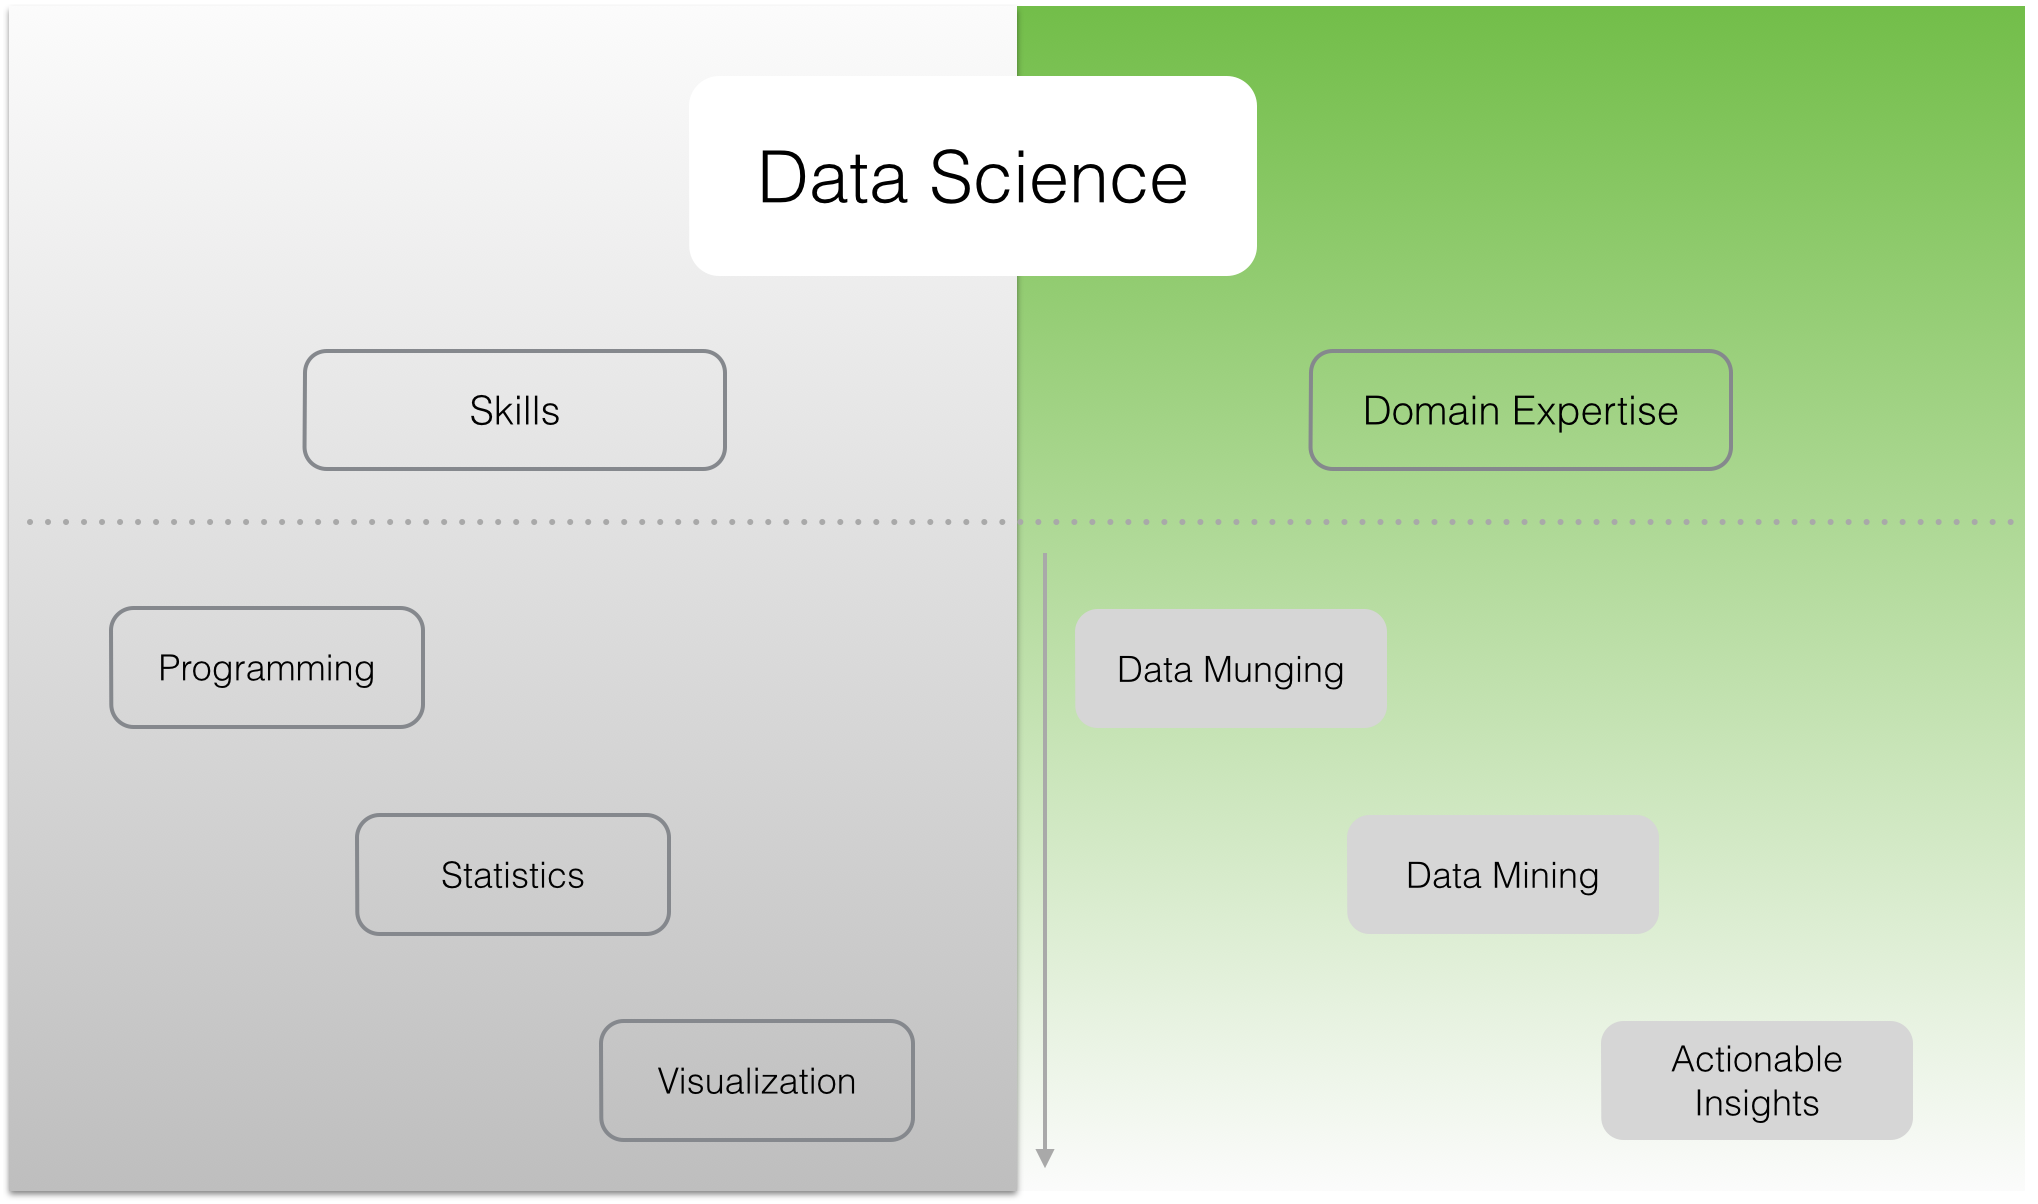
\includegraphics[width=300pt]{../graphs/data_science_structure}
      \end{center}
    \end{frame}

  \subsection{Data Munging}
  
   \begin{frame}{Data Munging}
     \begin{columns}
       \begin{column}[T]{0.48\textwidth}
         \begin{block}{Data Munging}
           ..also called Data Wrangling, Data Preparation, usually means some or all of the following tasks that mark the beginning of a data science project:
           \begin{itemize}
             \item<1-> ETL
             \item<2-> Data Integration
             \item<3-> Data Cleansing
           \end{itemize}
         \end{block}
       \end{column}
       \begin{column}[T]{0.48\textwidth}
         \begin{overprint}
           \onslide<1>
             \begin{alertblock}{ETL}
               ETL is the process of extract, transform, and load data. - For one thing, we might want to acquire data from external sources to assist with data mining. On the other hand, there are often multiple data sources internally.
             \end{alertblock}
           \onslide <2>
             \begin{alertblock}{Data Integration}
               After ETL, we need to combine data from disparate sources into meaningful and valuable information.
             \end{alertblock}
           \onslide <3>
             \begin{alertblock}{Data Cleansing}
               Data cleansing, also called data scrubbing, is the process of amending or removing data in a database that is incorrect, incomplete, improperly formatted, or duplicated.
             \end{alertblock}
         \end{overprint}
       \end{column}   
     \end{columns}
   \end{frame}

  \subsection{Skills and Domain Expertise}

    \begin{frame}{Domain expertise of a data scientist}
      \begin{center}
        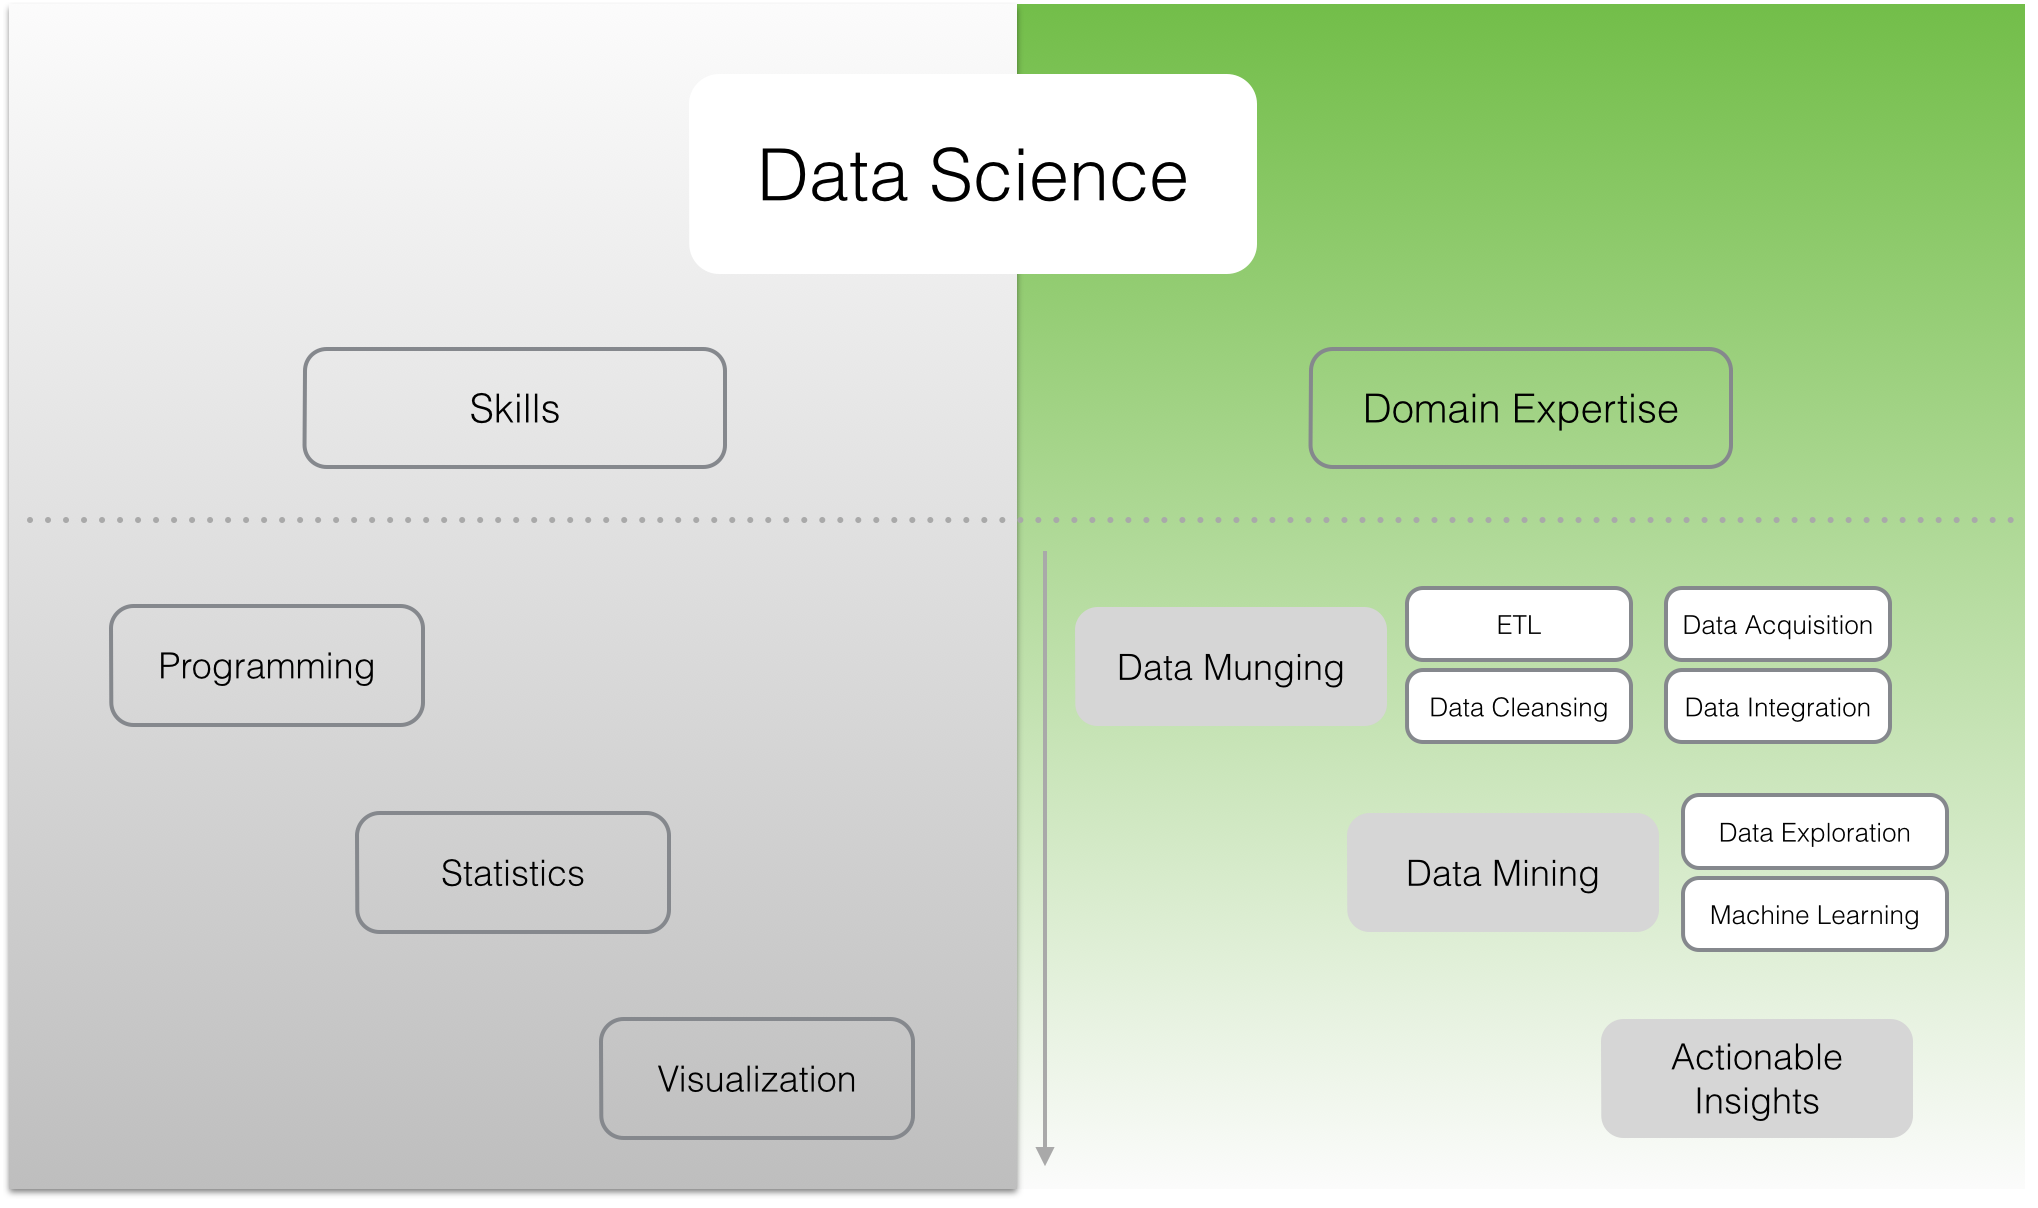
\includegraphics[width=300pt]{../graphs/data_science_domain}
      \end{center}
    \end{frame}

    \begin{frame}{Skills of a data scientist}
      \begin{center}
        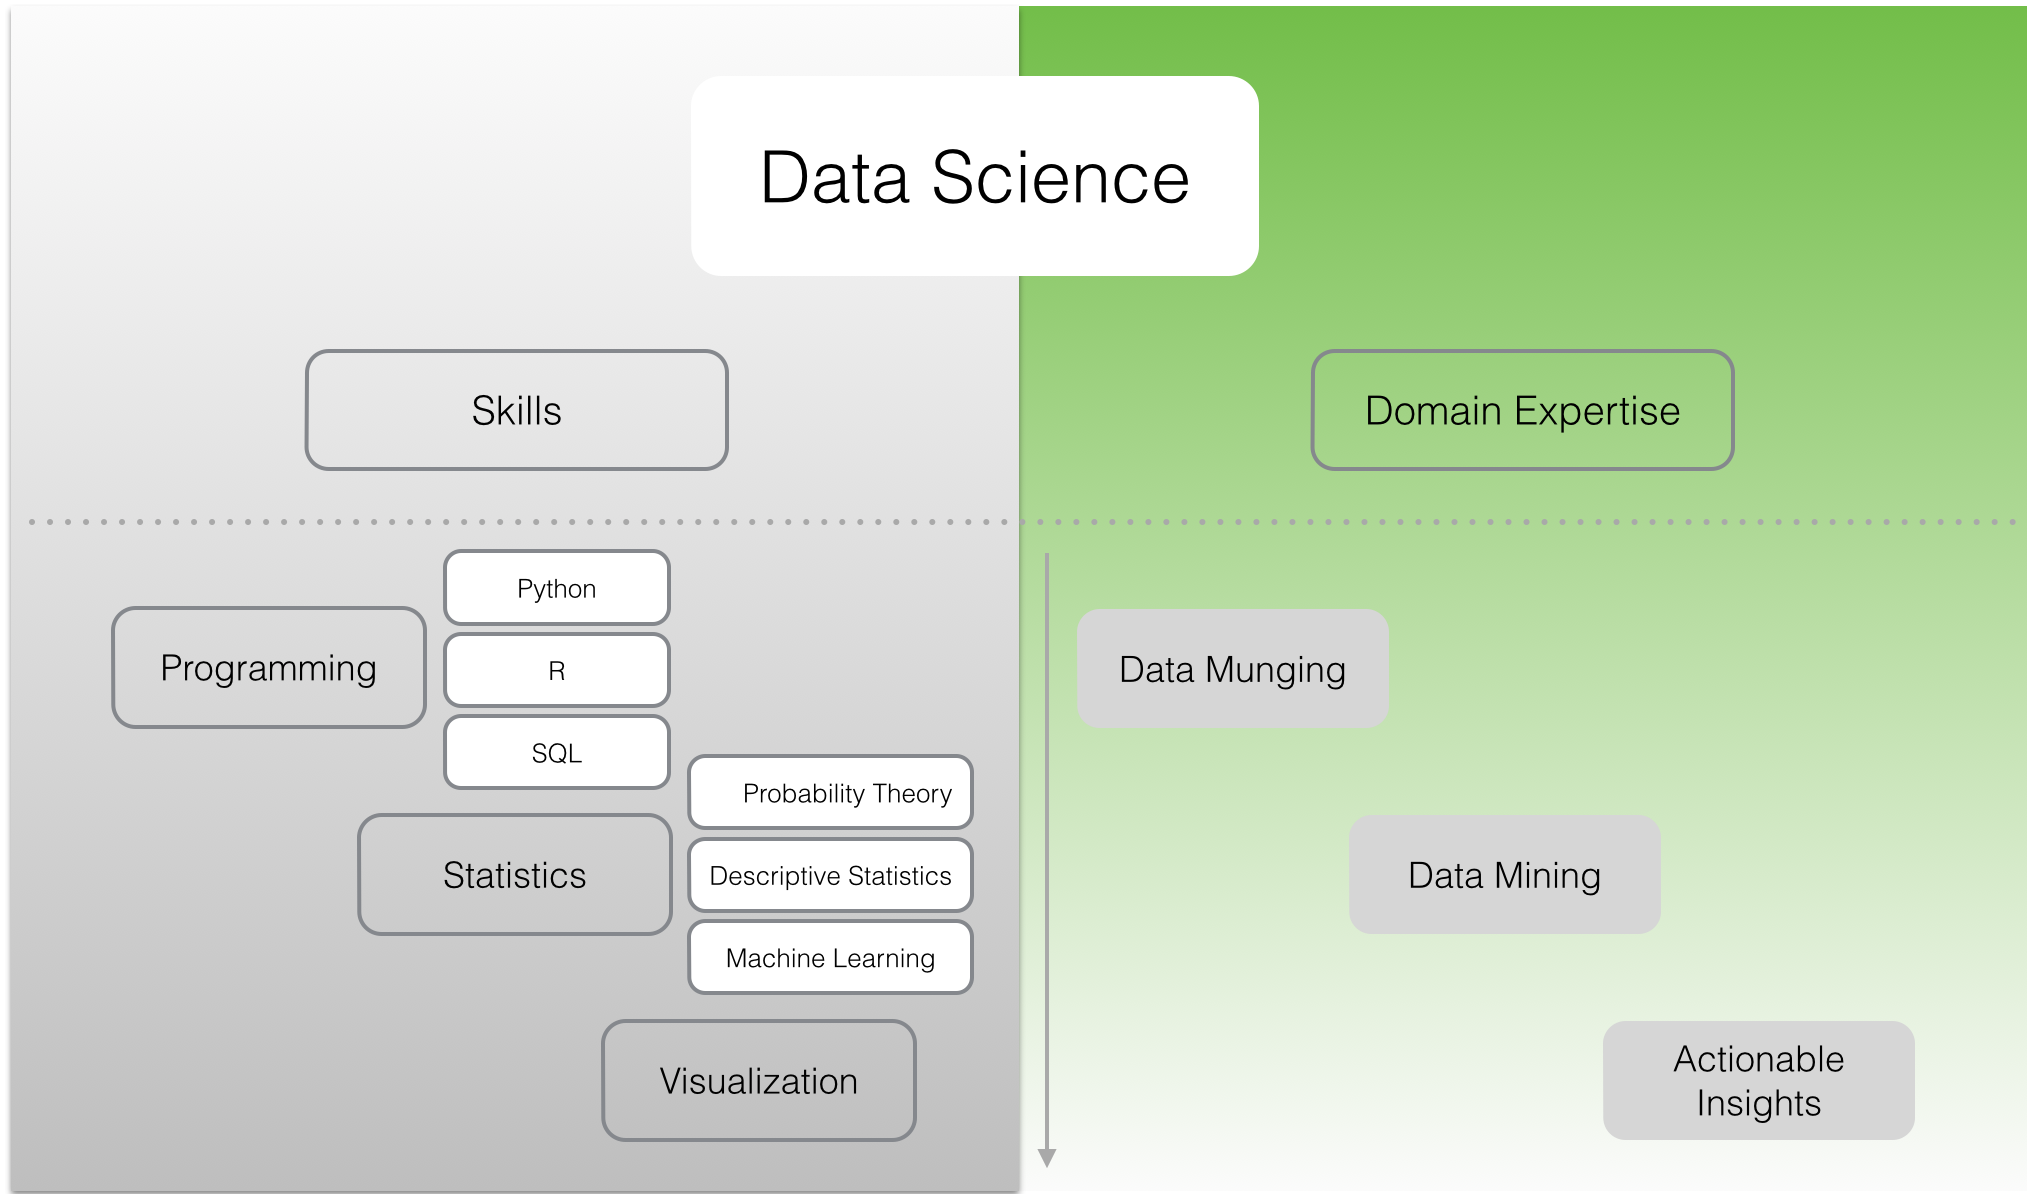
\includegraphics[width=300pt]{../graphs/data_science_skills}
      \end{center}
    \end{frame}

    \begin{frame}{Doing data science}
      \begin{center}
        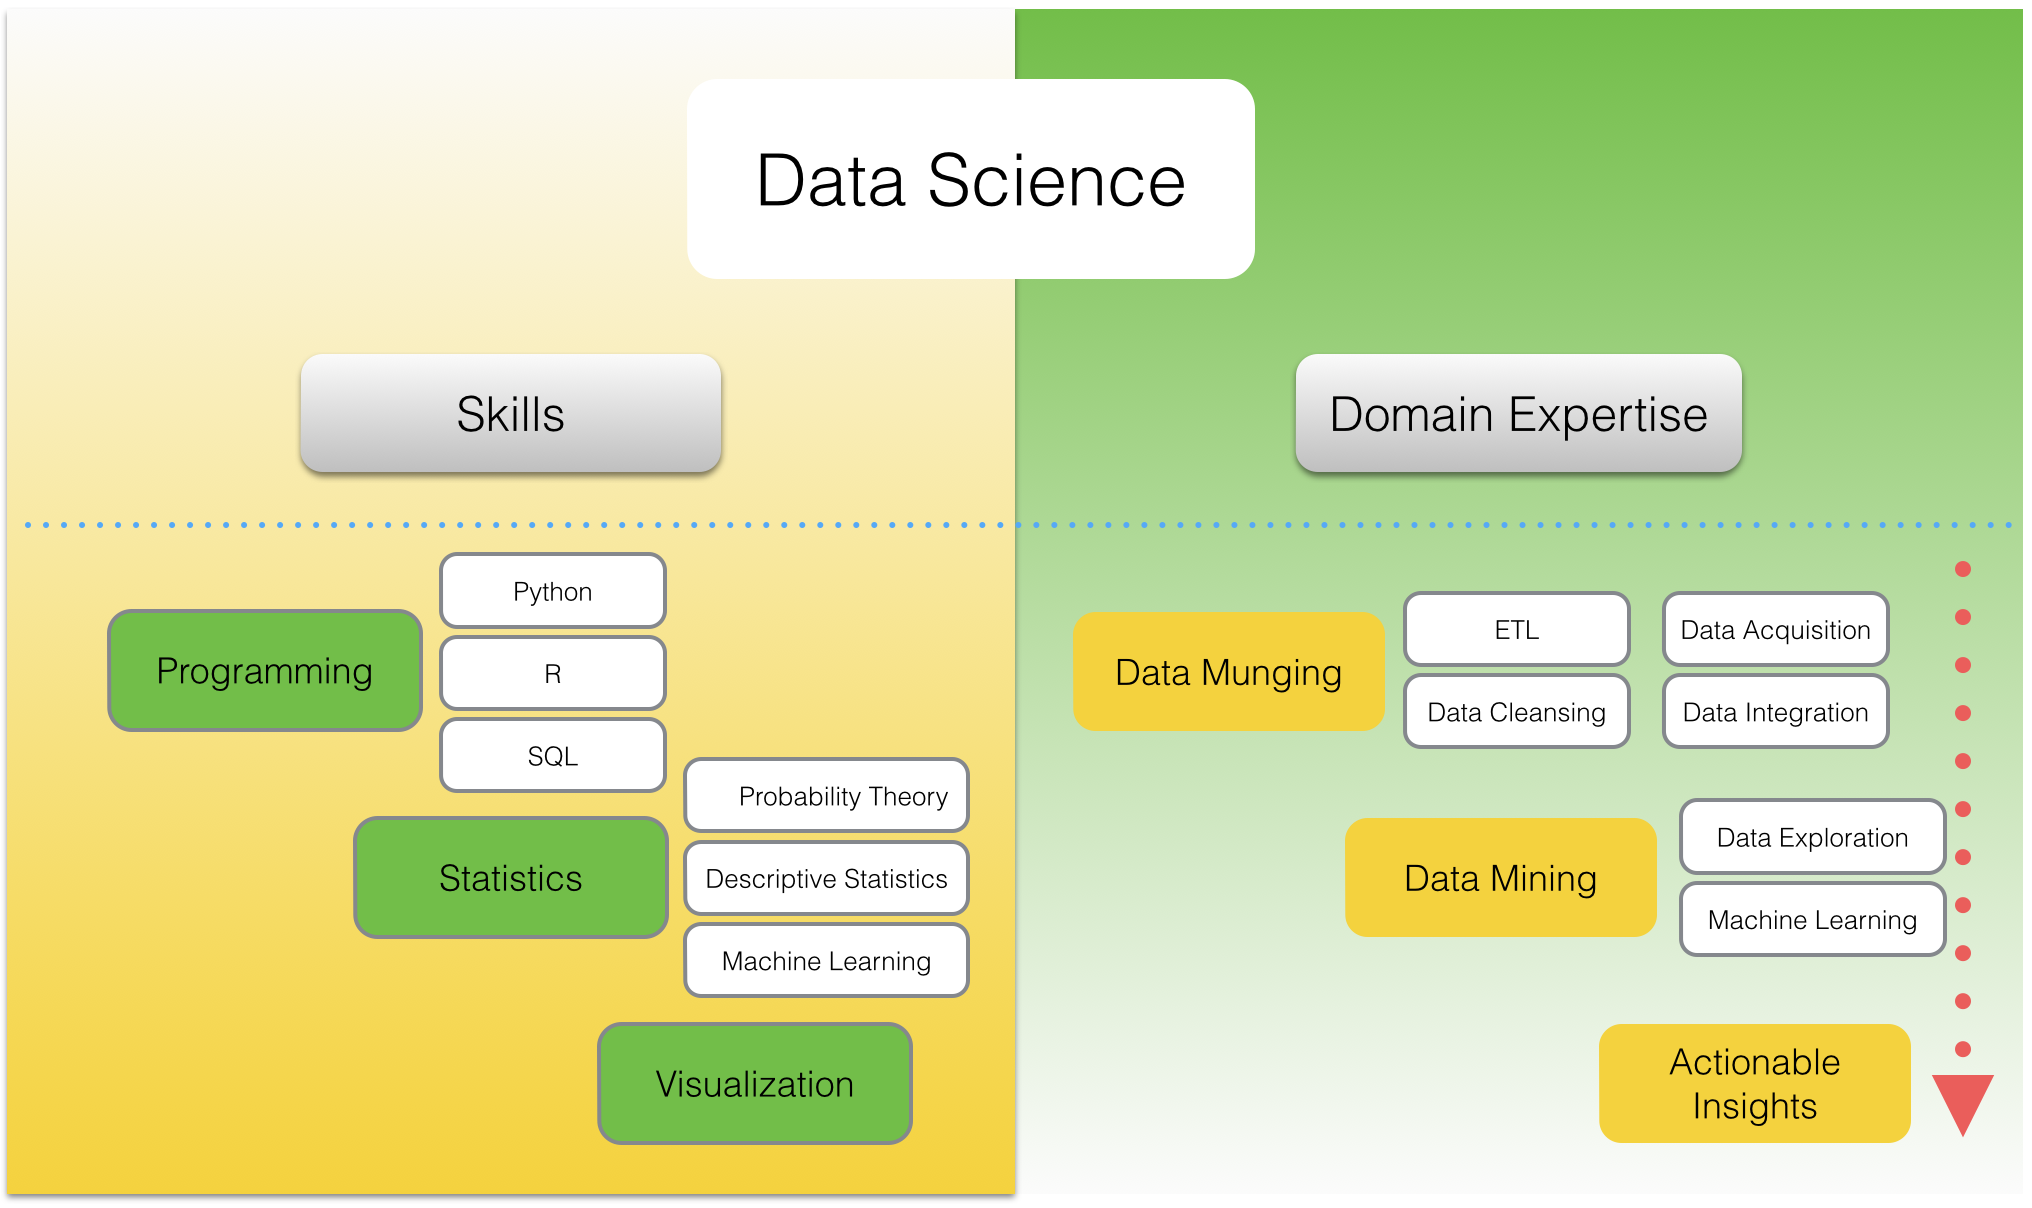
\includegraphics[width=300pt]{../graphs/data_science_skills_domain}
      \end{center}
    \end{frame}

\section{Churn Model}

  \subsection{Business Understanding}

      \begin{frame}{The Goal}
        \begin{block}{Goal}
            \begin{itemize}
              \item To predict which customers will churn.
            \end{itemize}
        \end{block}
        \begin{block}{Workflow}
          \begin{center}
            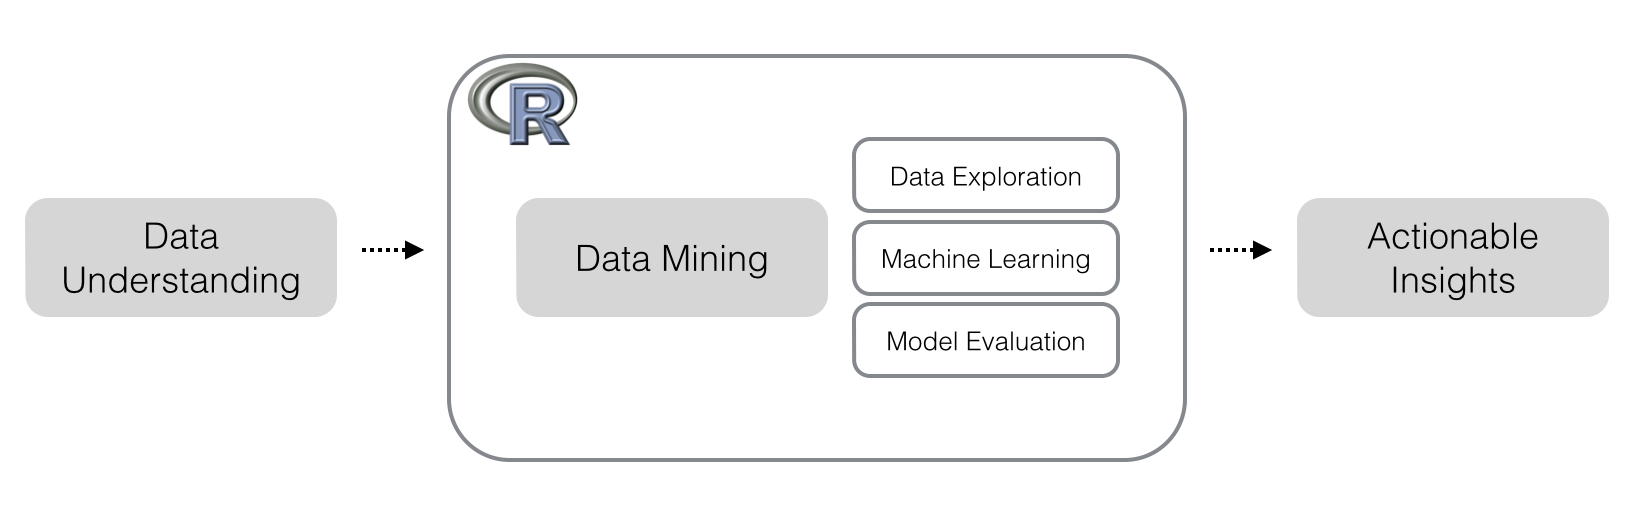
\includegraphics[height=80pt]{../graphs/churnmodel_workflow}
          \end{center}
        \end{block}
      \end{frame}

    \begin{frame}{Customer renewal data}
      \begin{center}
        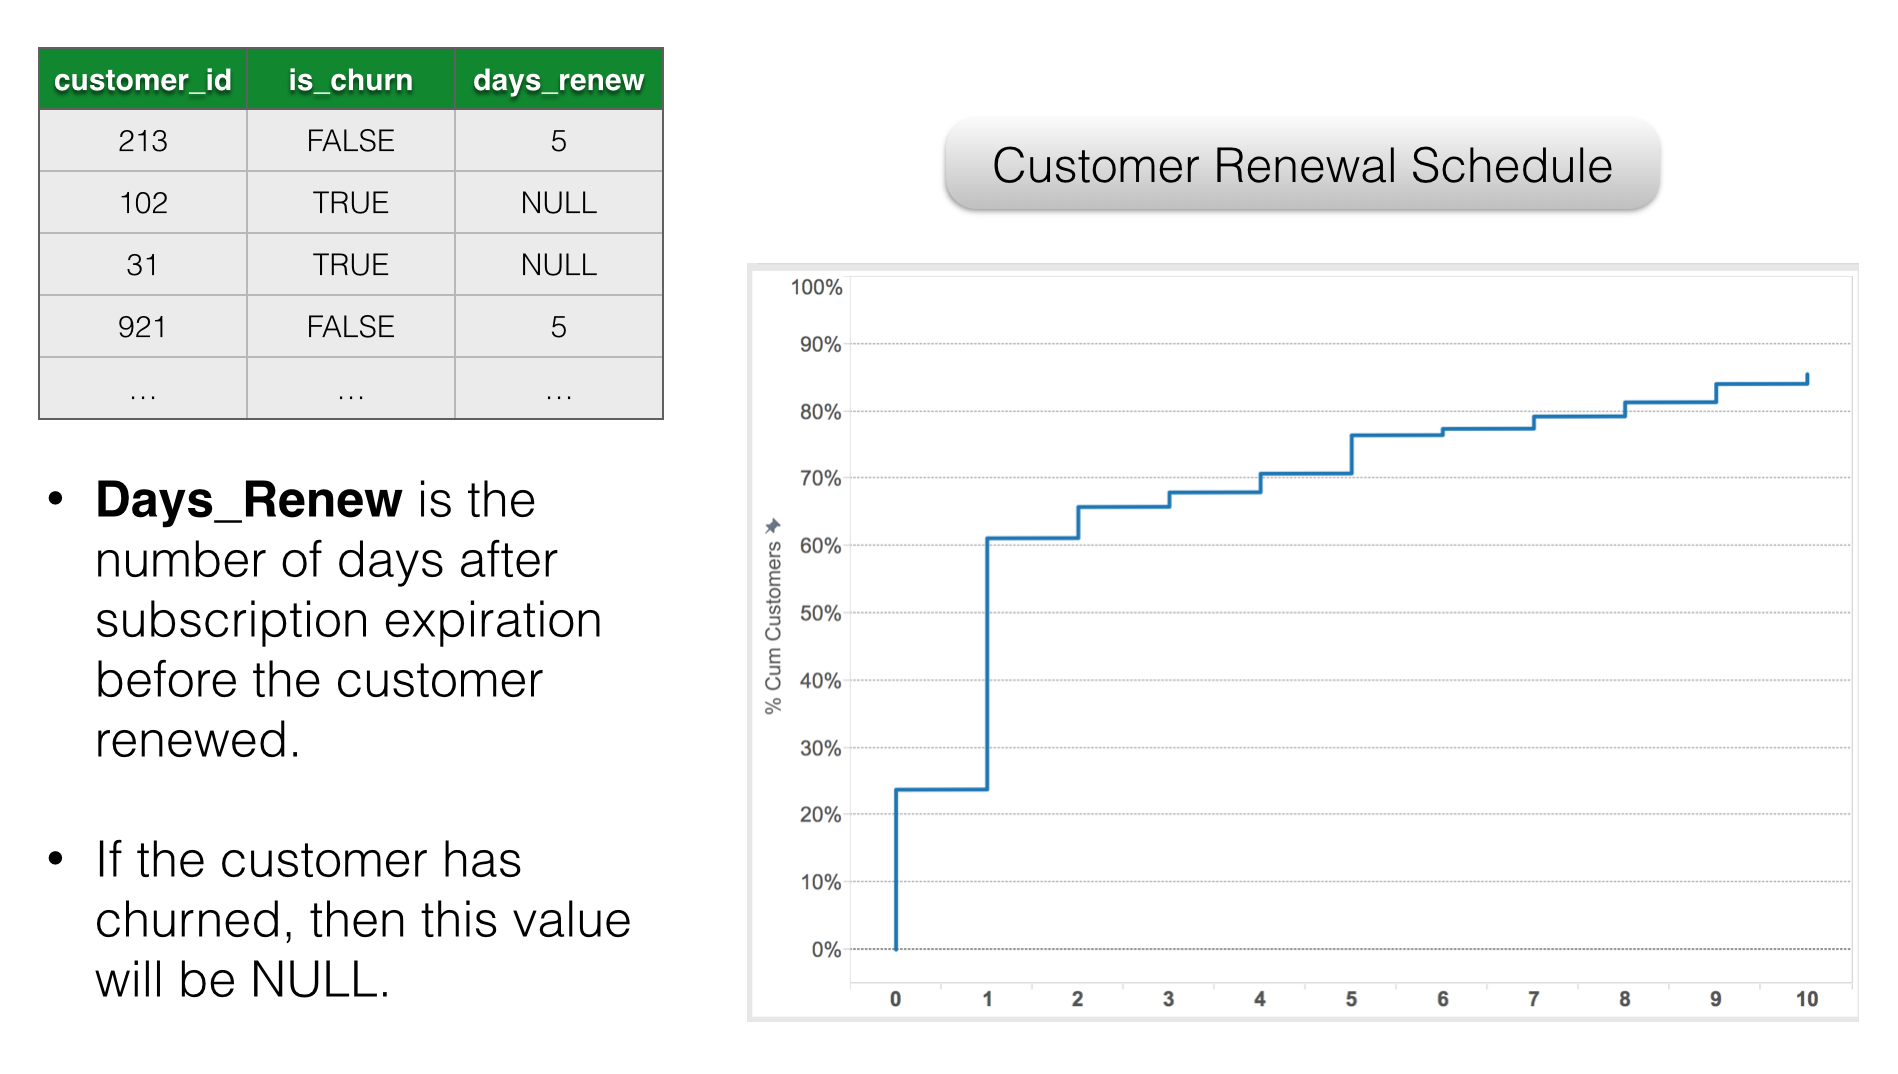
\includegraphics[height=180pt]{../graphs/datasets_customer_renew}
      \end{center}
    \end{frame}

    \begin{frame}{Customer service call data}
      \begin{center}
        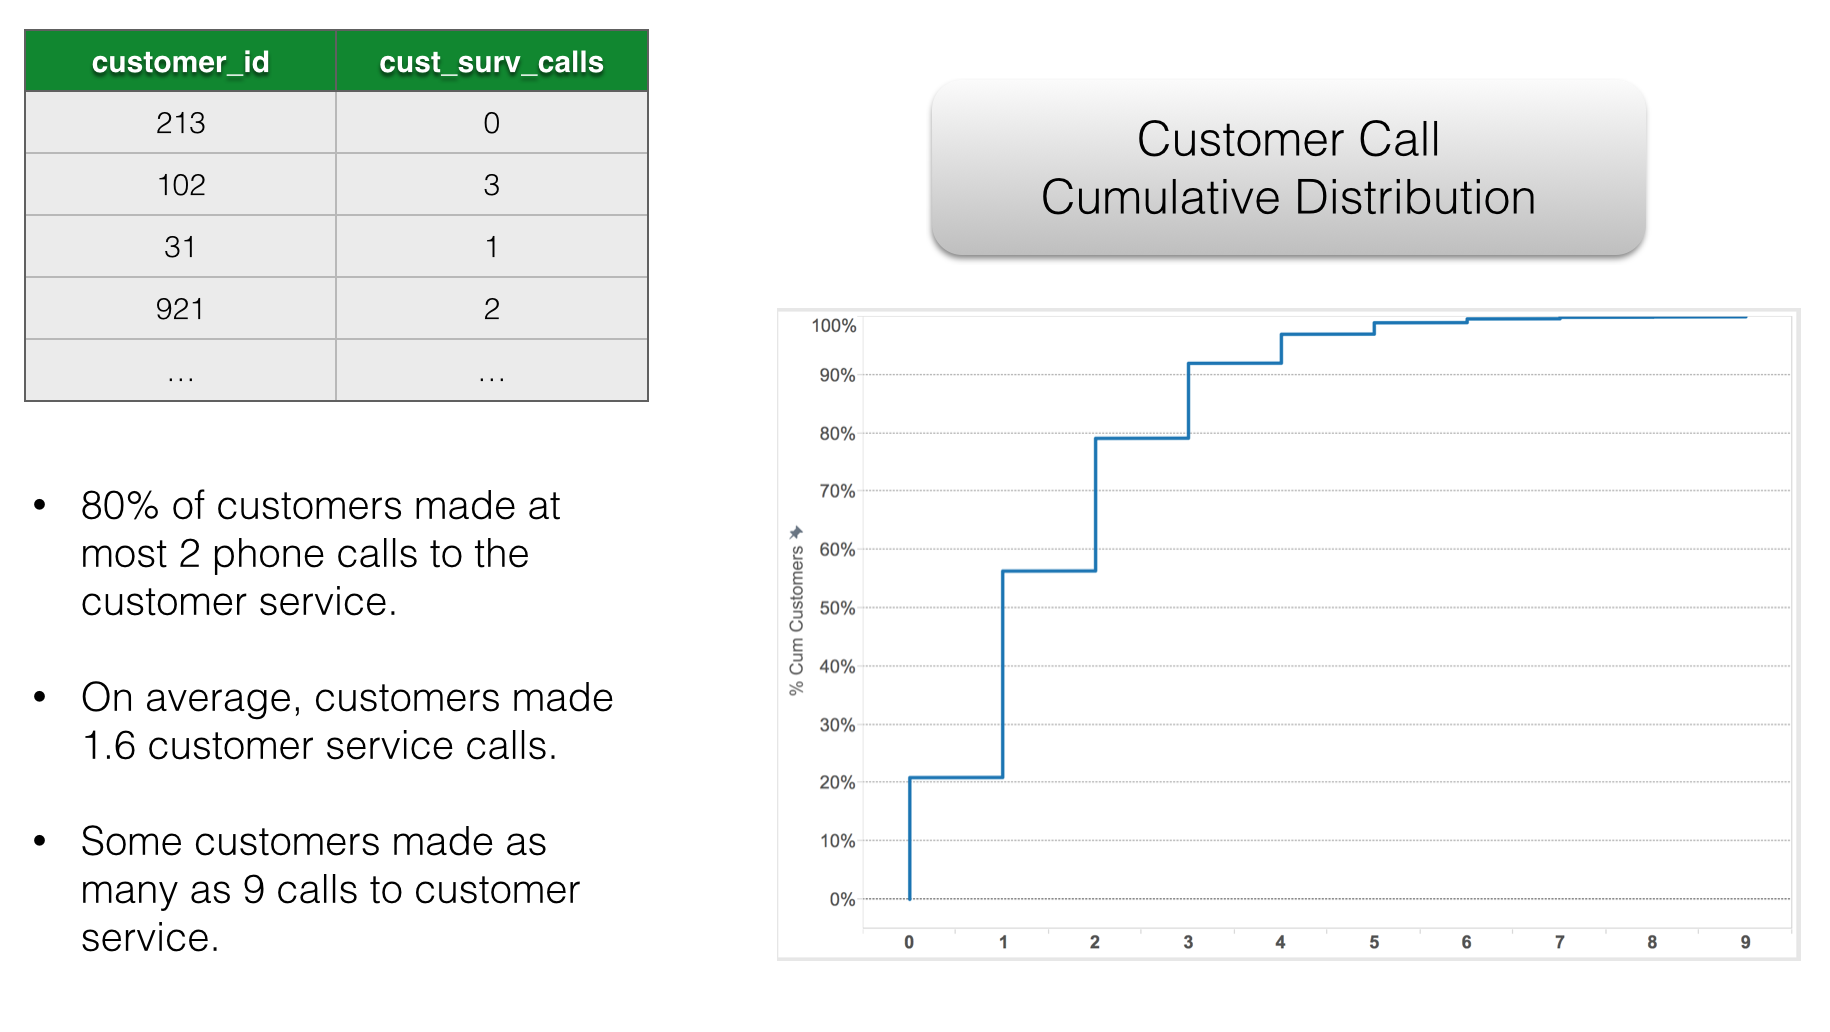
\includegraphics[height=180pt]{../graphs/datasets_cust_call}
      \end{center}
    \end{frame}

    \begin{frame}{Customer plan type and demographic}
        \begin{center}
          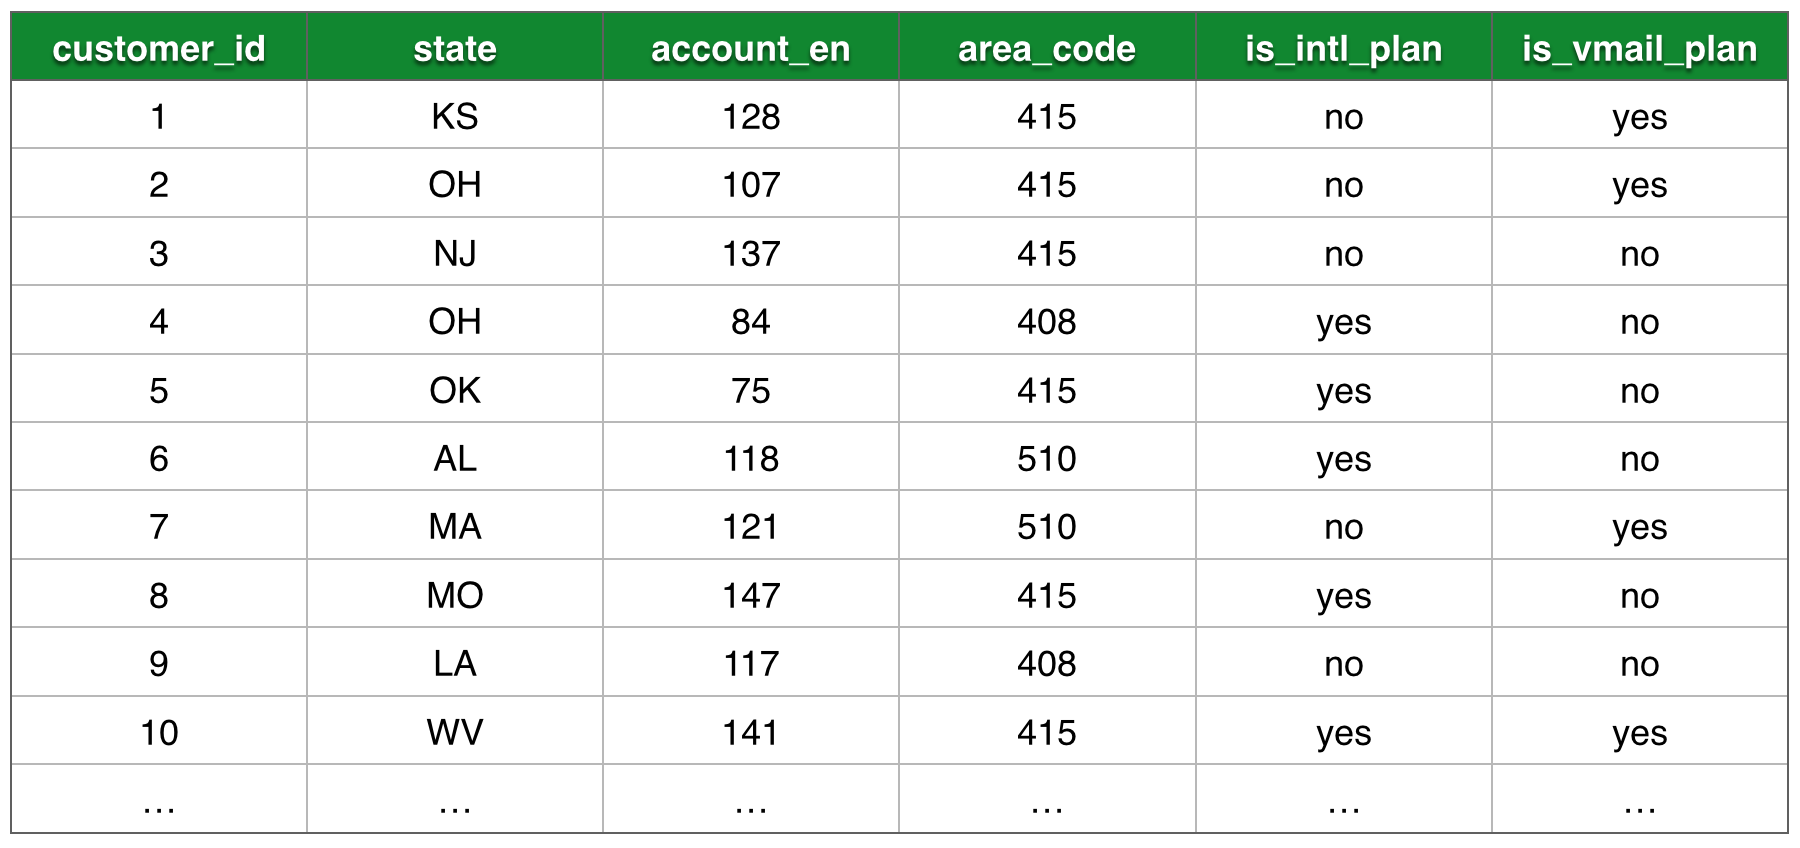
\includegraphics[height=150pt]{../graphs/datasets_customer_account}
        \end{center}
    \end{frame}

    \begin{frame}{Customer usage data}
        \begin{center}
          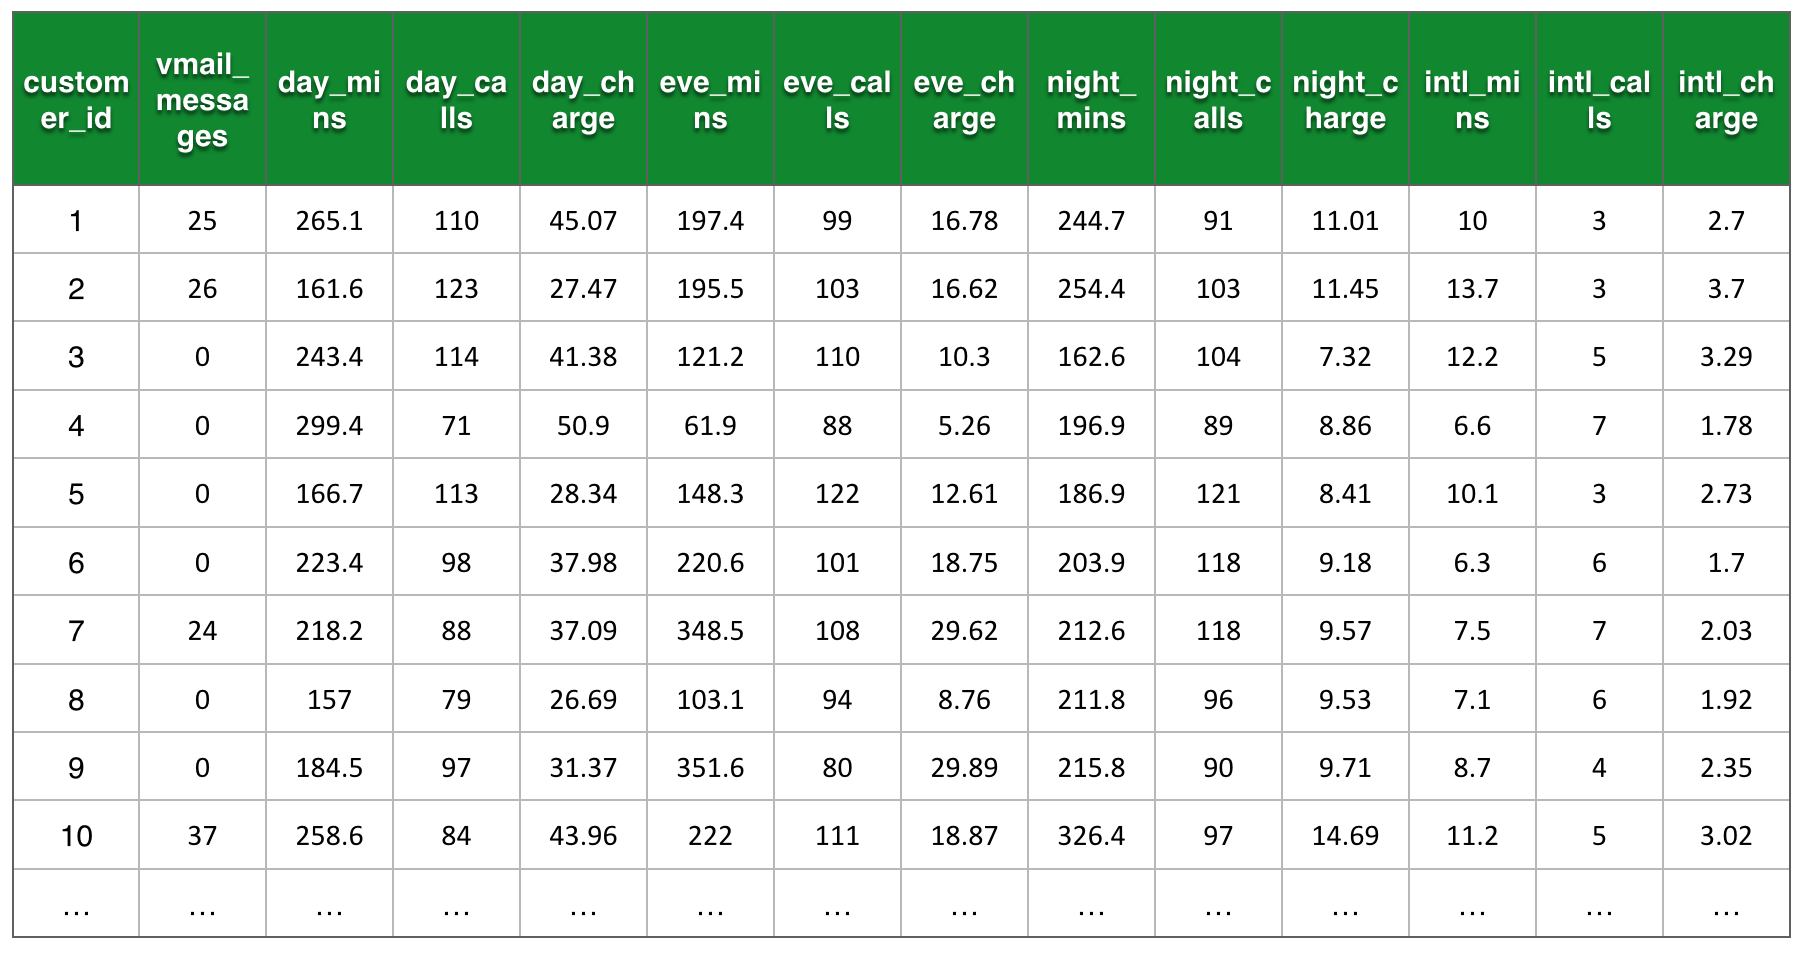
\includegraphics[height=150pt]{../graphs/datasets_customer_usage}
        \end{center}
    \end{frame}

    \begin{frame}{Churn data structure}
      \begin{center}
        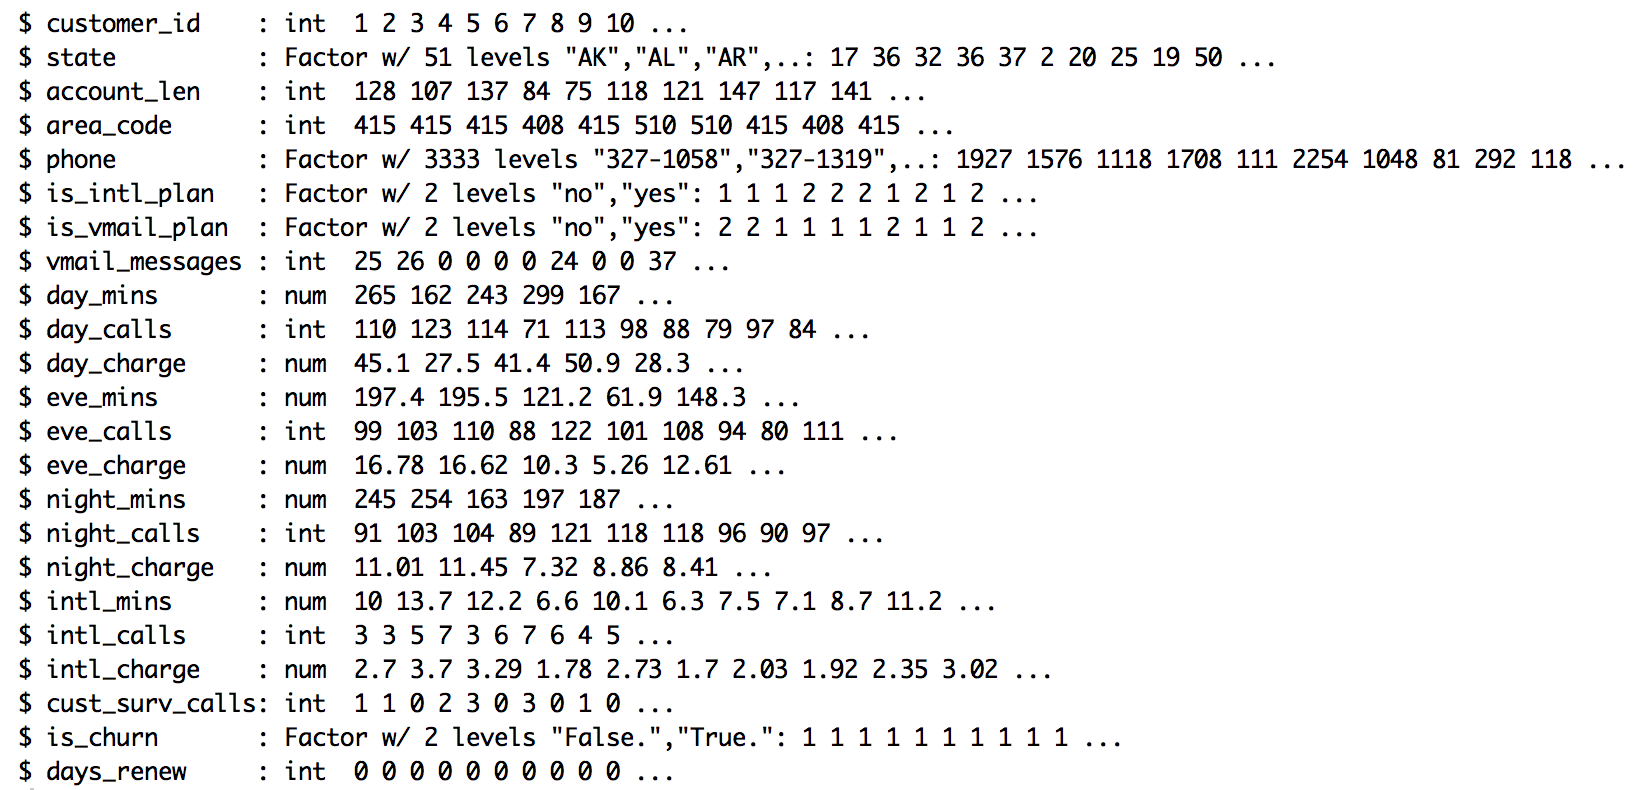
\includegraphics[height=180pt]{../graphs/dataset_churn_str}
      \end{center}
    \end{frame}

  \subsection{Demo in R}

    \begin{frame}{R Script}
        \begin{center}
          {\large \url{https://github.com/vieplivee/Data-Science-in-Action/blob/master/src/churn.R}}
        \end{center}
    \end{frame}
    
  \subsection{Top Features}
  
    \begin{frame}{Variable importance from random forest}
        \begin{center}
          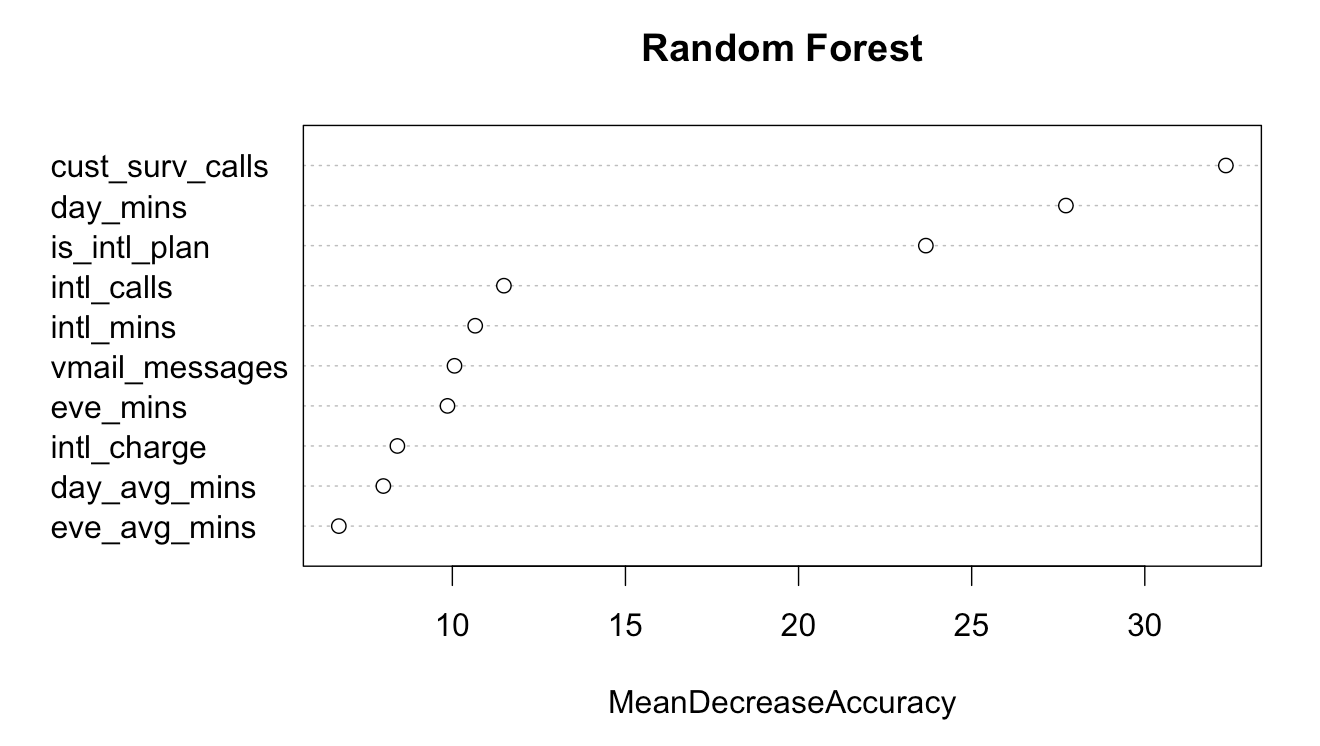
\includegraphics[width=300pt]{../graphs/rf_var_importance}
        \end{center}
    \end{frame}

    \begin{frame}{Top feature - customer service calls}
      \begin{center}
        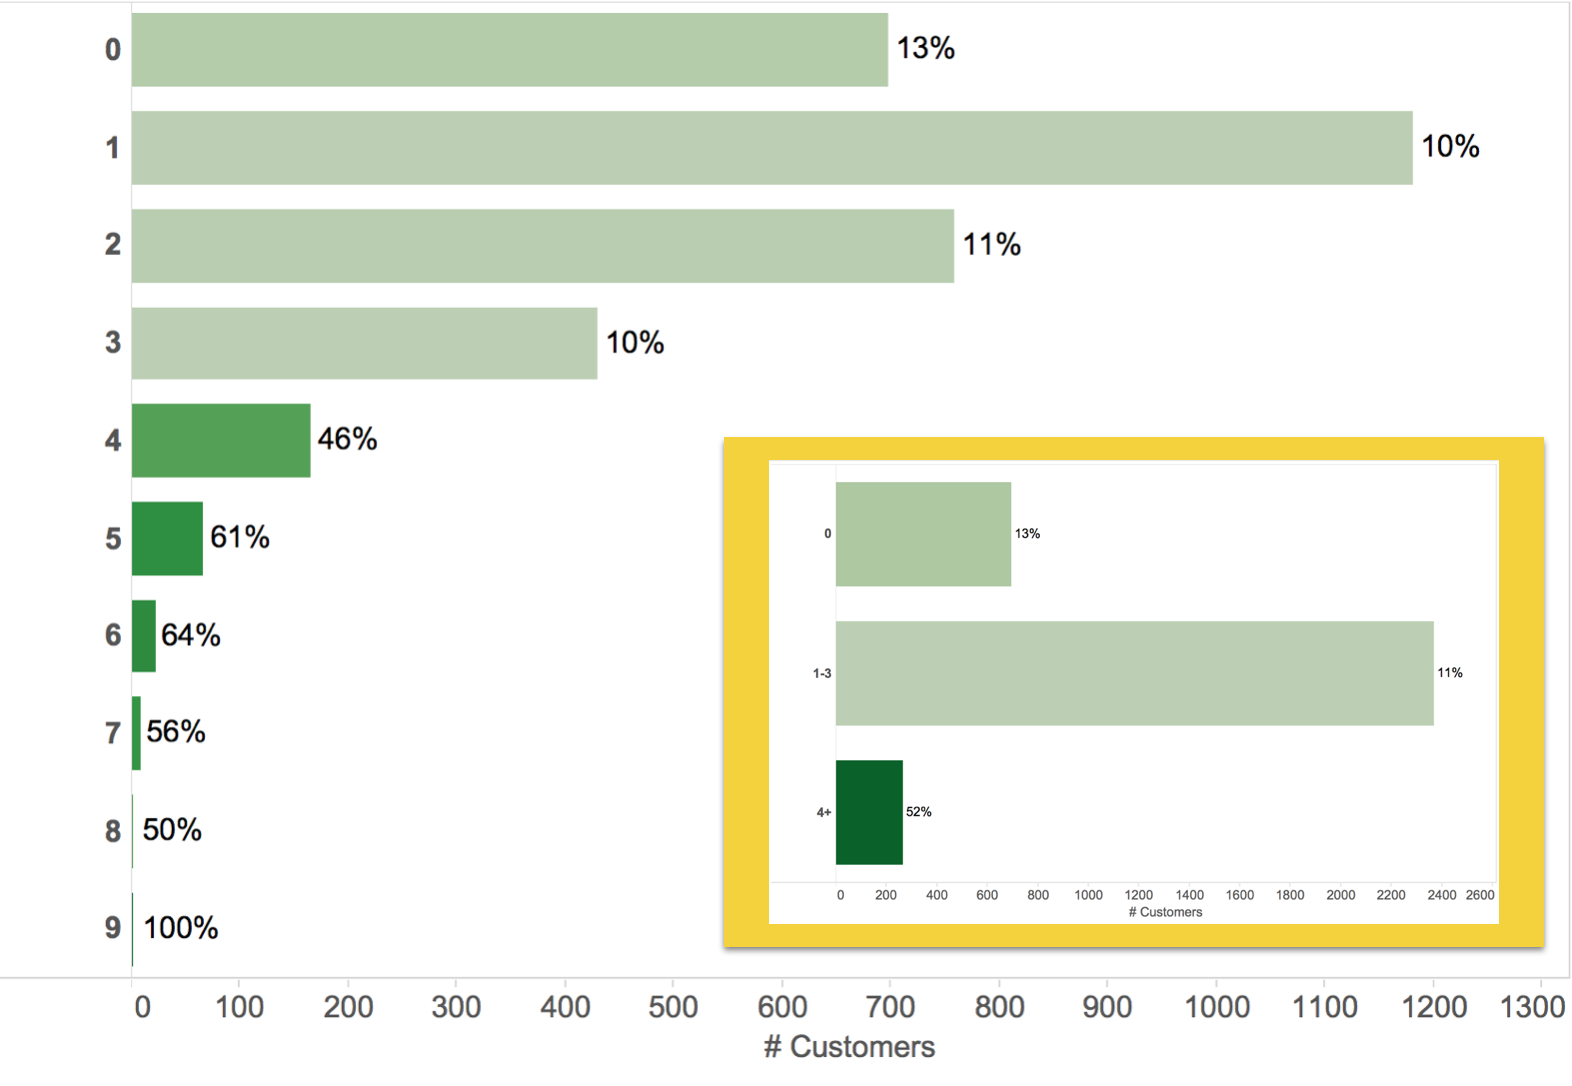
\includegraphics[width=280pt]{../graphs/top_var_cust_surv_with_group}
      \end{center}
    \end{frame}

    \begin{frame}{Top feature - customer day time minutes}
      \begin{center}
        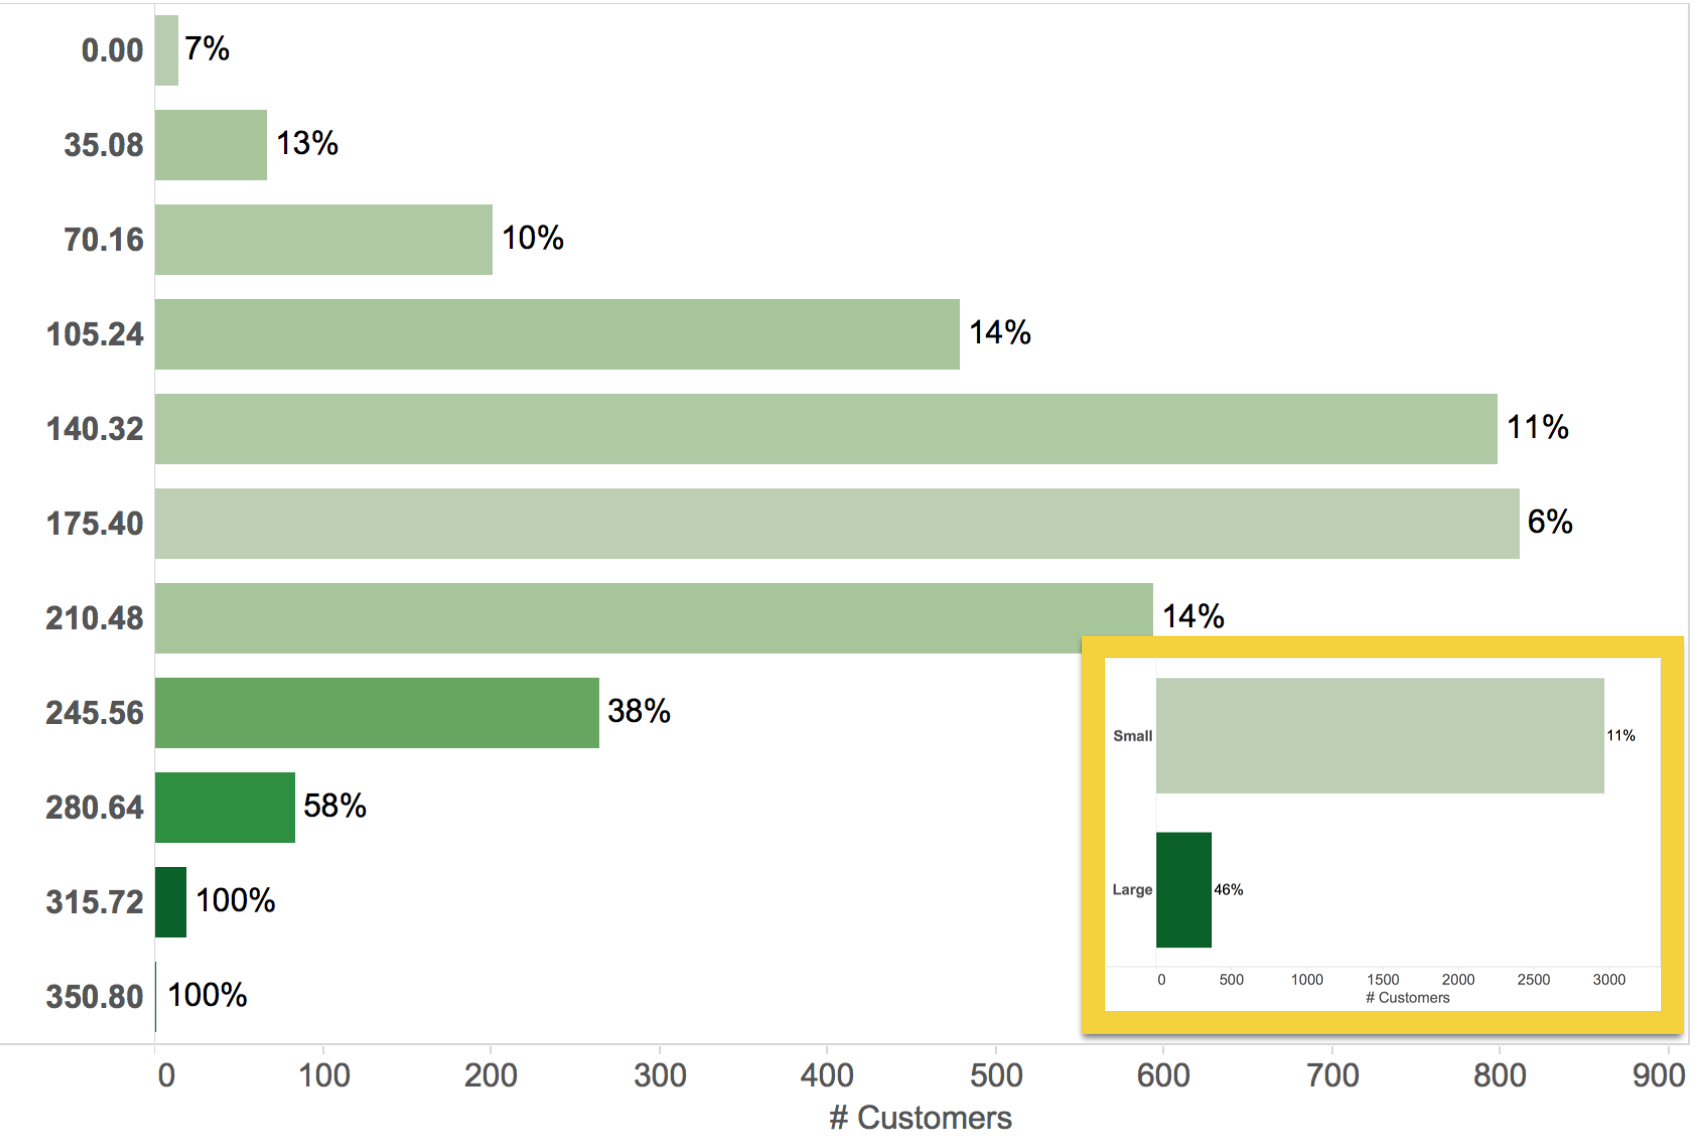
\includegraphics[width=280pt]{../graphs/top_var_day_mins_with_group}
      \end{center}
    \end{frame}

    \begin{frame}{Top feature - international plan and international calls}
      \begin{center}
        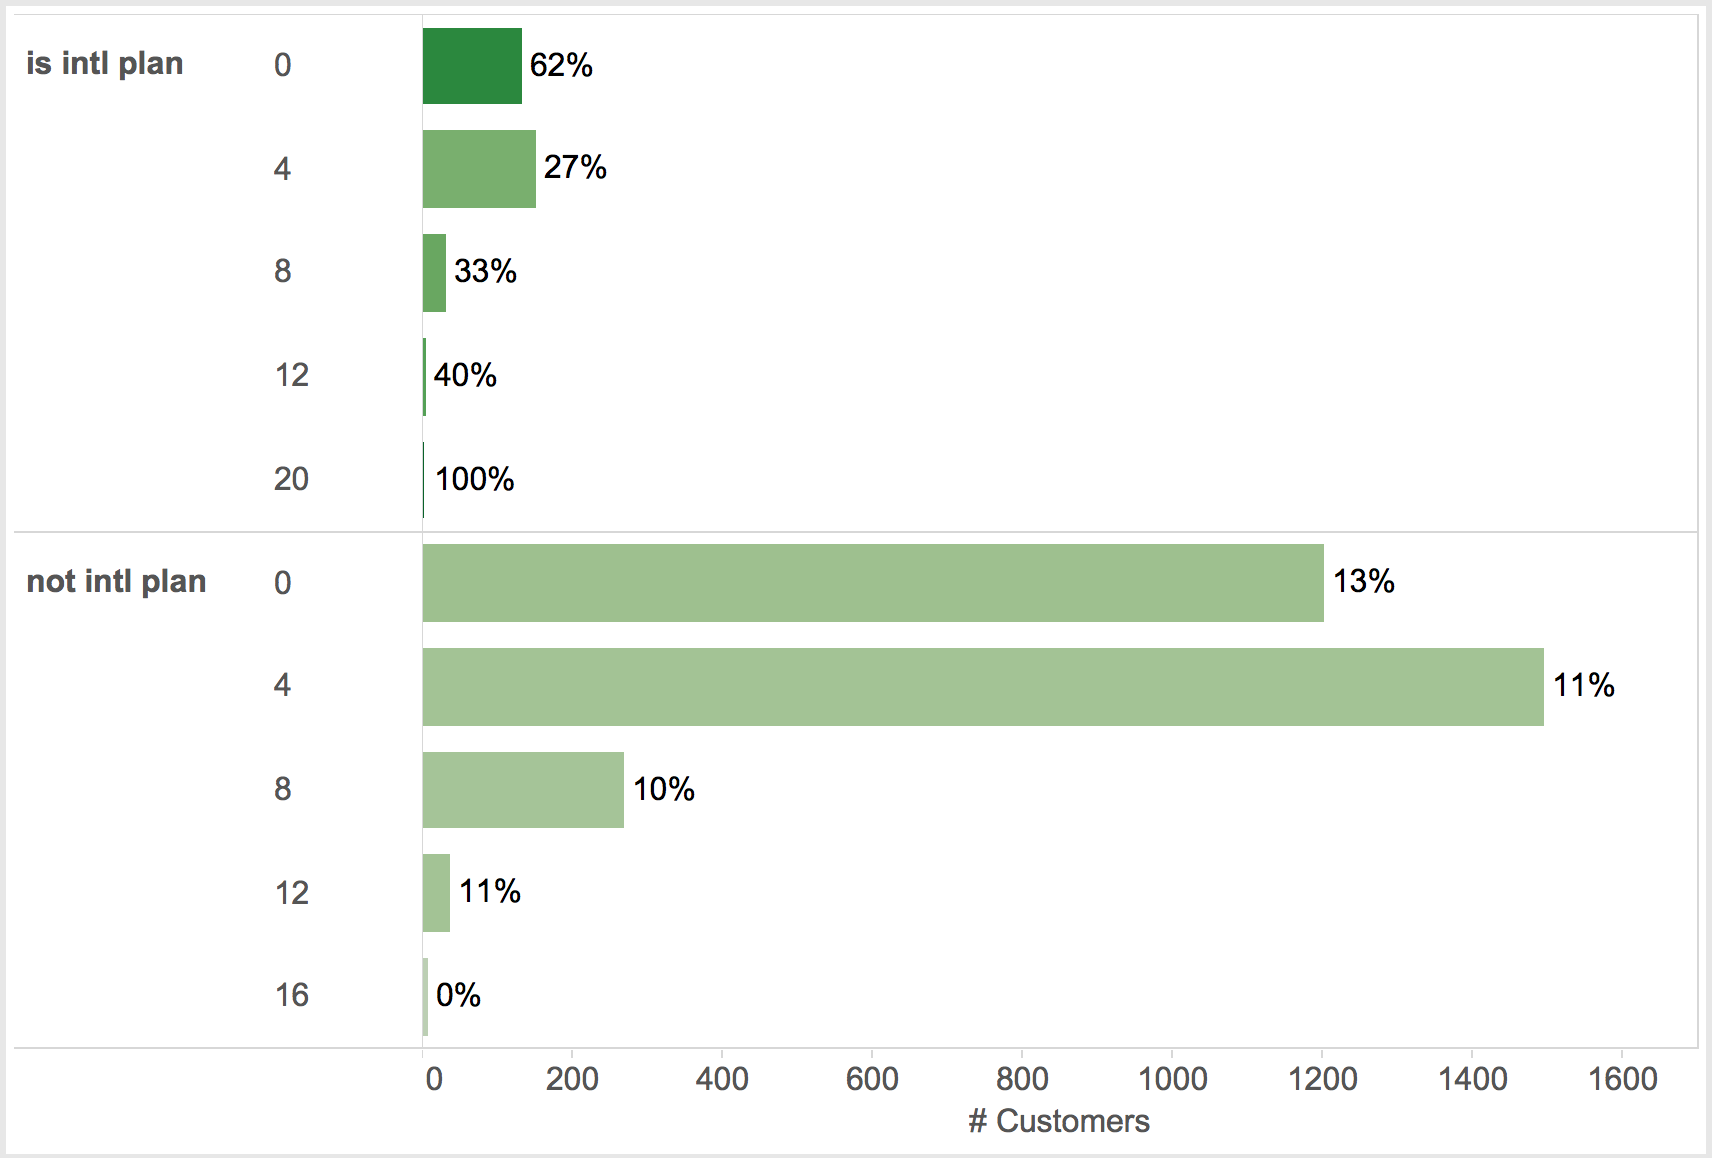
\includegraphics[width=280pt]{../graphs/top_var_intl_plan_calls}
      \end{center}
    \end{frame}

  \subsection{Prescriptive Analysis}

    \begin{frame}{Churn analysis}
      \begin{center}
        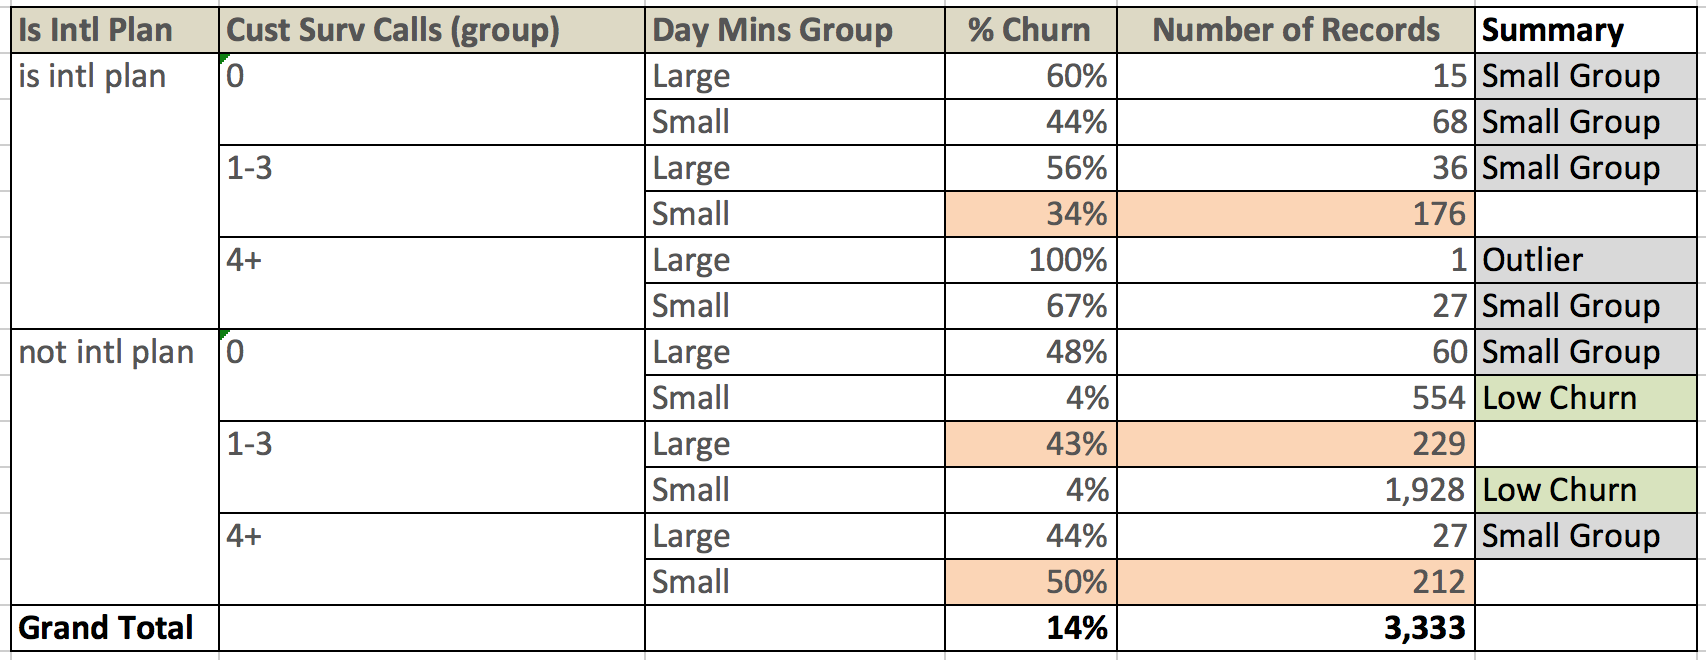
\includegraphics[height=120pt]{../graphs/churn_analysis}
      \end{center}
    \end{frame}

    \begin{frame}{Churn analysis}
      \begin{center}
        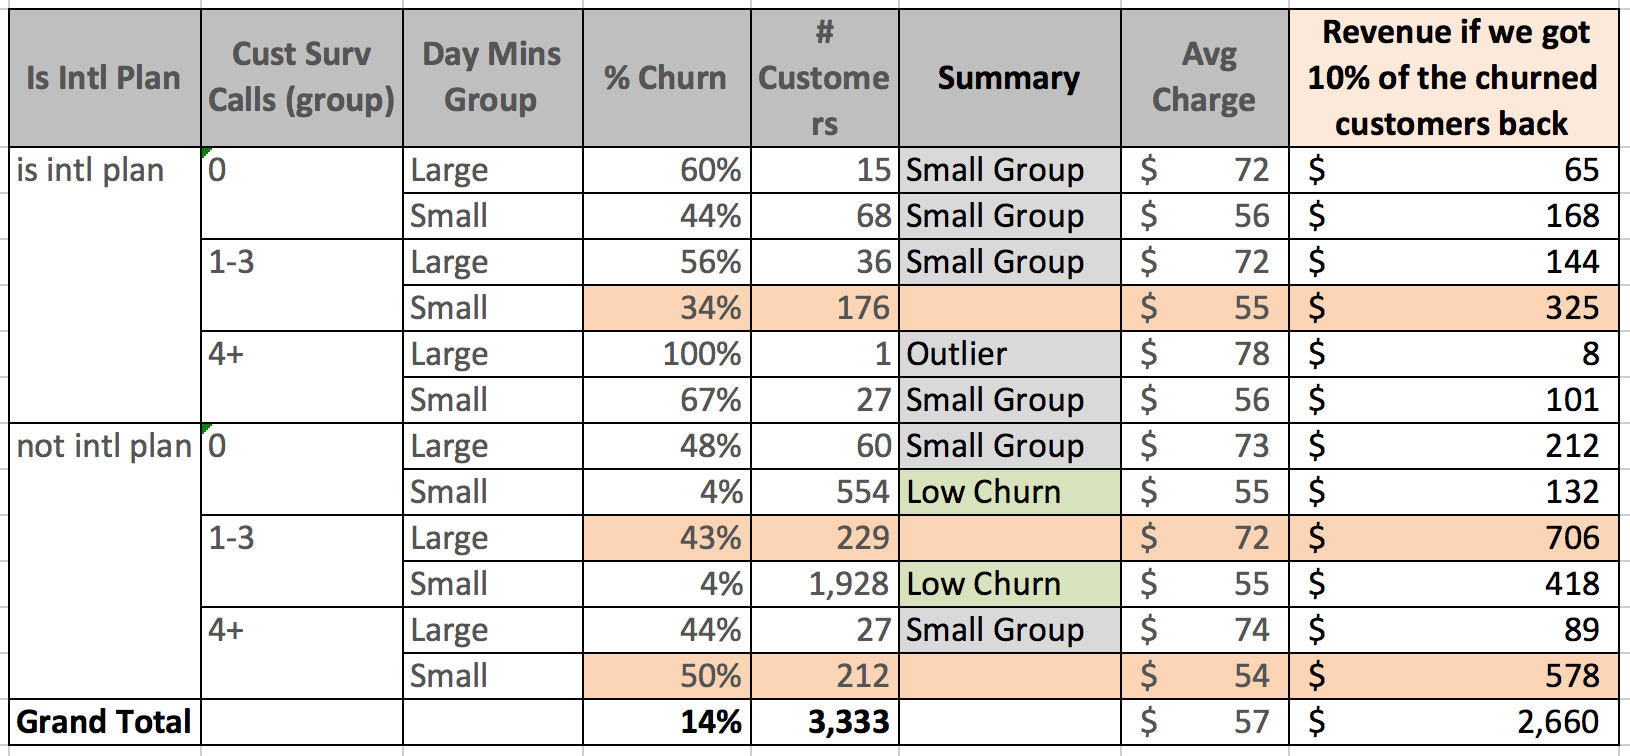
\includegraphics[height=150pt]{../graphs/churn_analysis_revenue}
      \end{center}
    \end{frame}

\section{Yesware Email Analysis}

  \subsection{Email Analysis}

    \begin{frame}{When to send an email}
      \begin{center}
        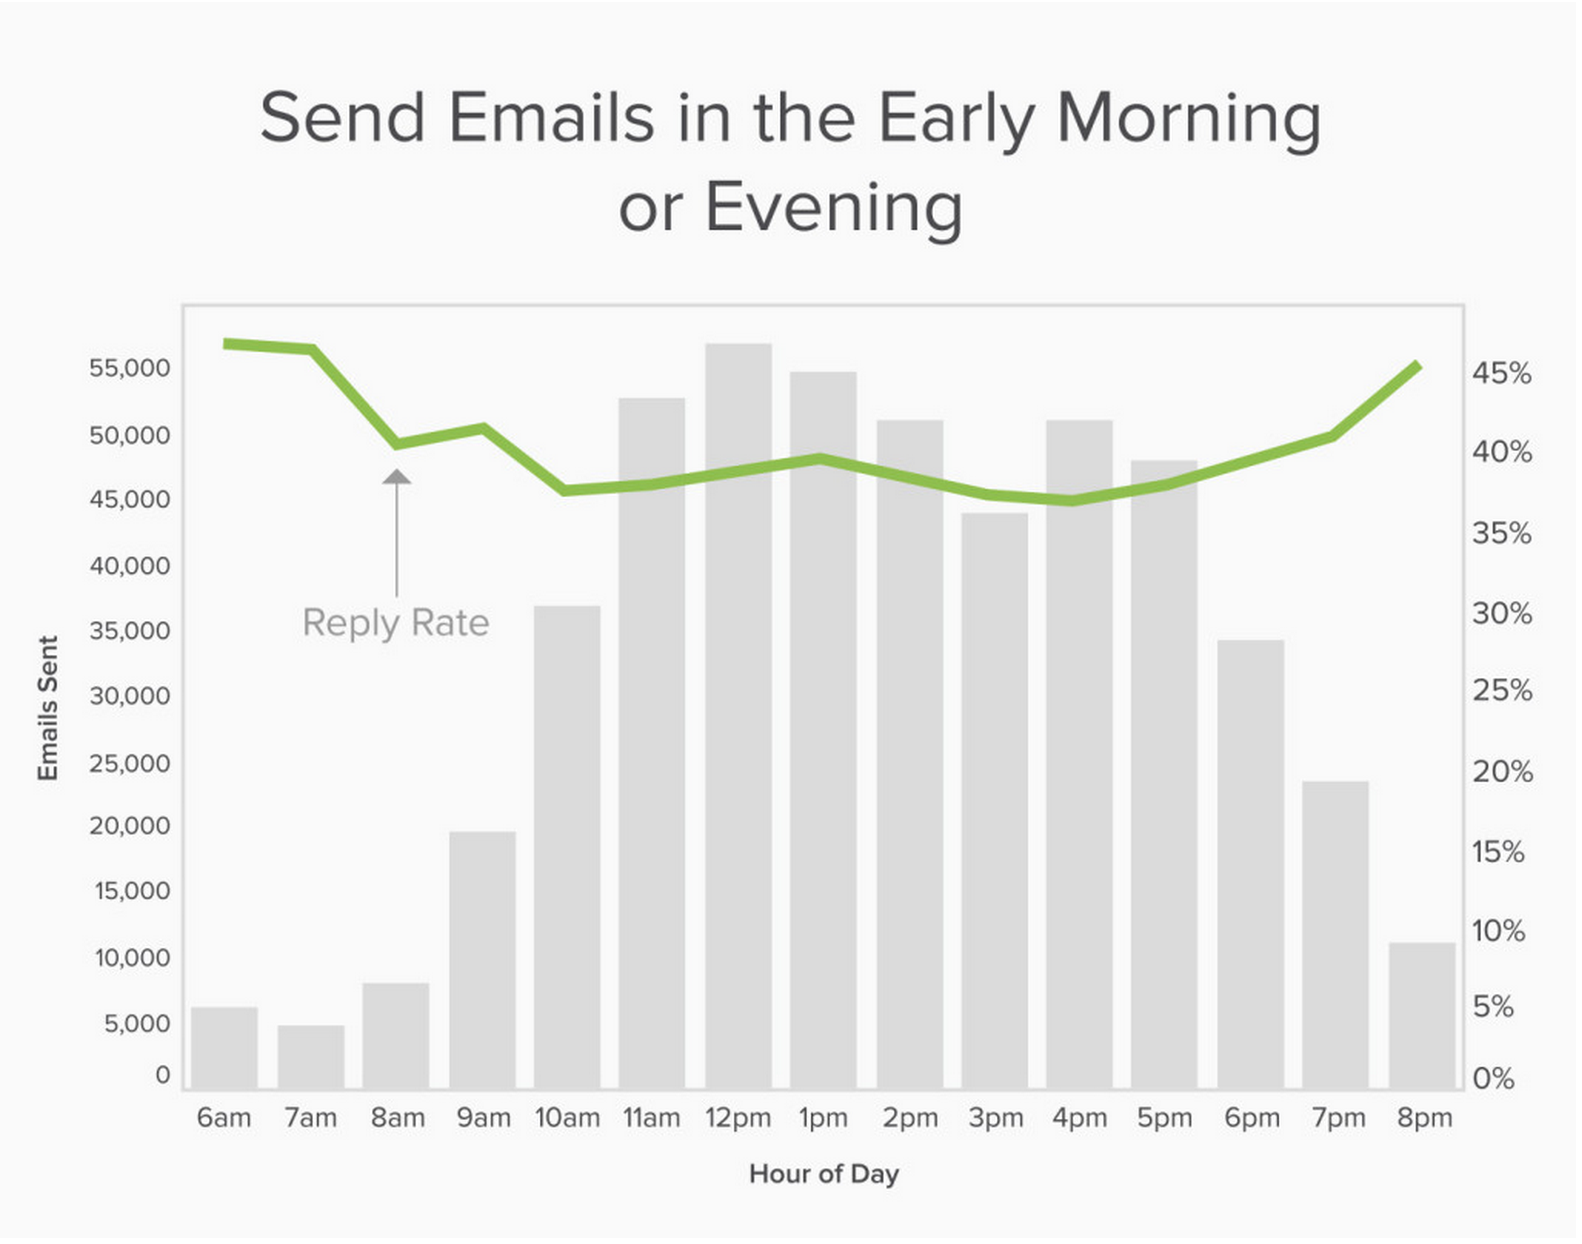
\includegraphics[height=180pt]{../graphs/email_analysis_sent_hour}
      \end{center}    
      {\footnotesize Best time to send email: \url{http://goo.gl/lVdD31}}
    \end{frame}

    \begin{frame}{D3 Visualization: Subject Line Keywords}
      \begin{center}
        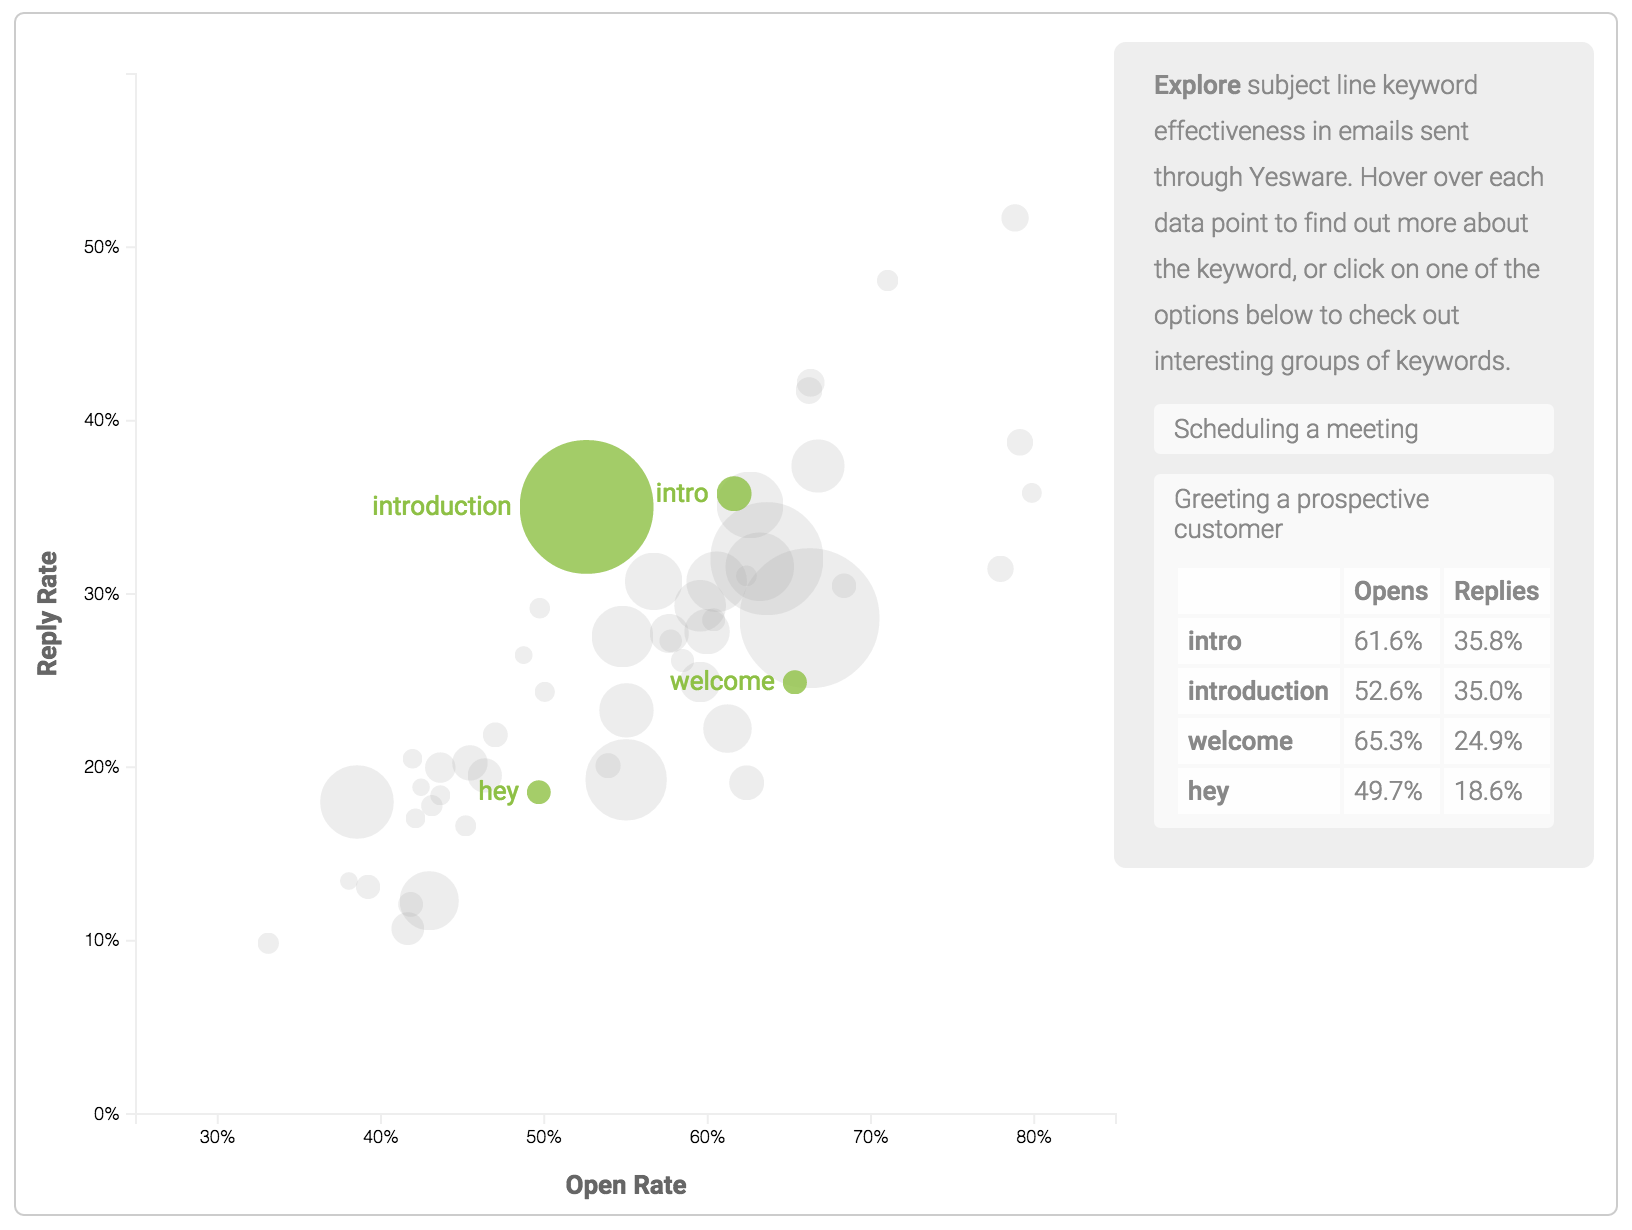
\includegraphics[height=180pt]{../graphs/email_analysis_subject_line}
      \end{center}    
      {\footnotesize Subject line key words: \url{http://goo.gl/PK9xhO}}
    \end{frame}

\section{Data Science in the Industry}

  \subsection{Data Science Toolbox}
  
    \begin{frame}{From academia to industry}
      \begin{center}
        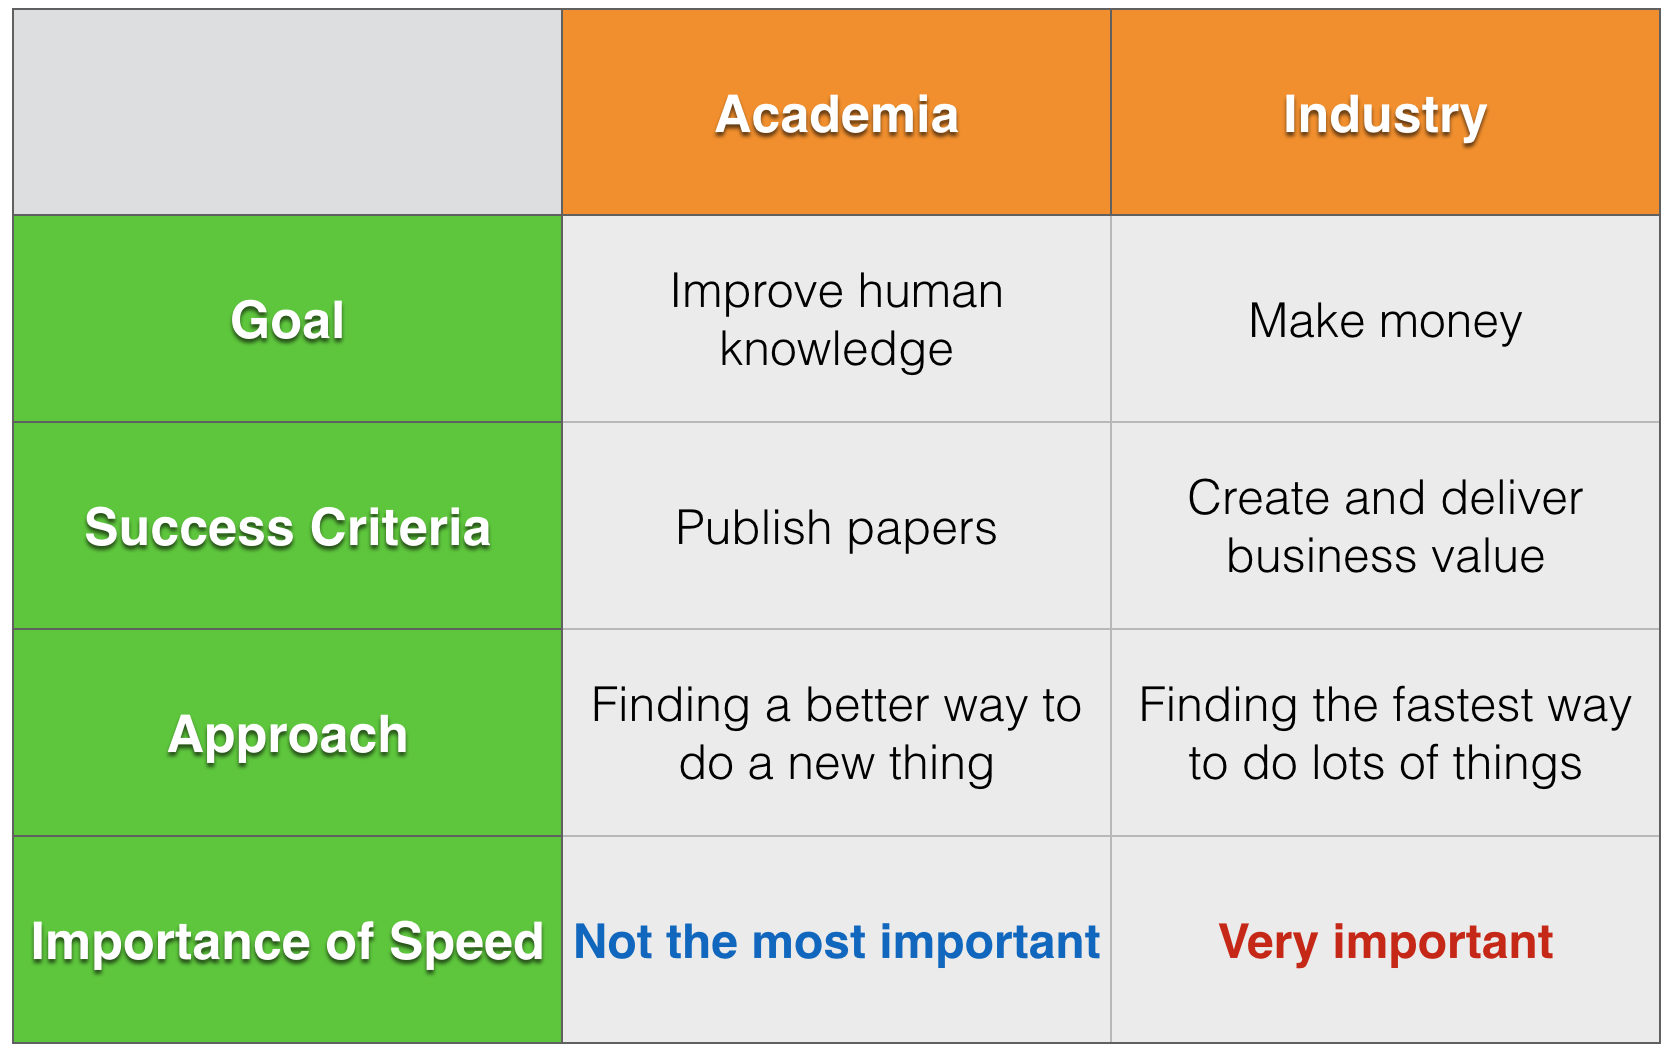
\includegraphics[width=300pt]{../graphs/academia_industry}
      \end{center}
    \end{frame}
    
    \begin{frame}{Tools that help you do data science fast}
      \begin{center}
         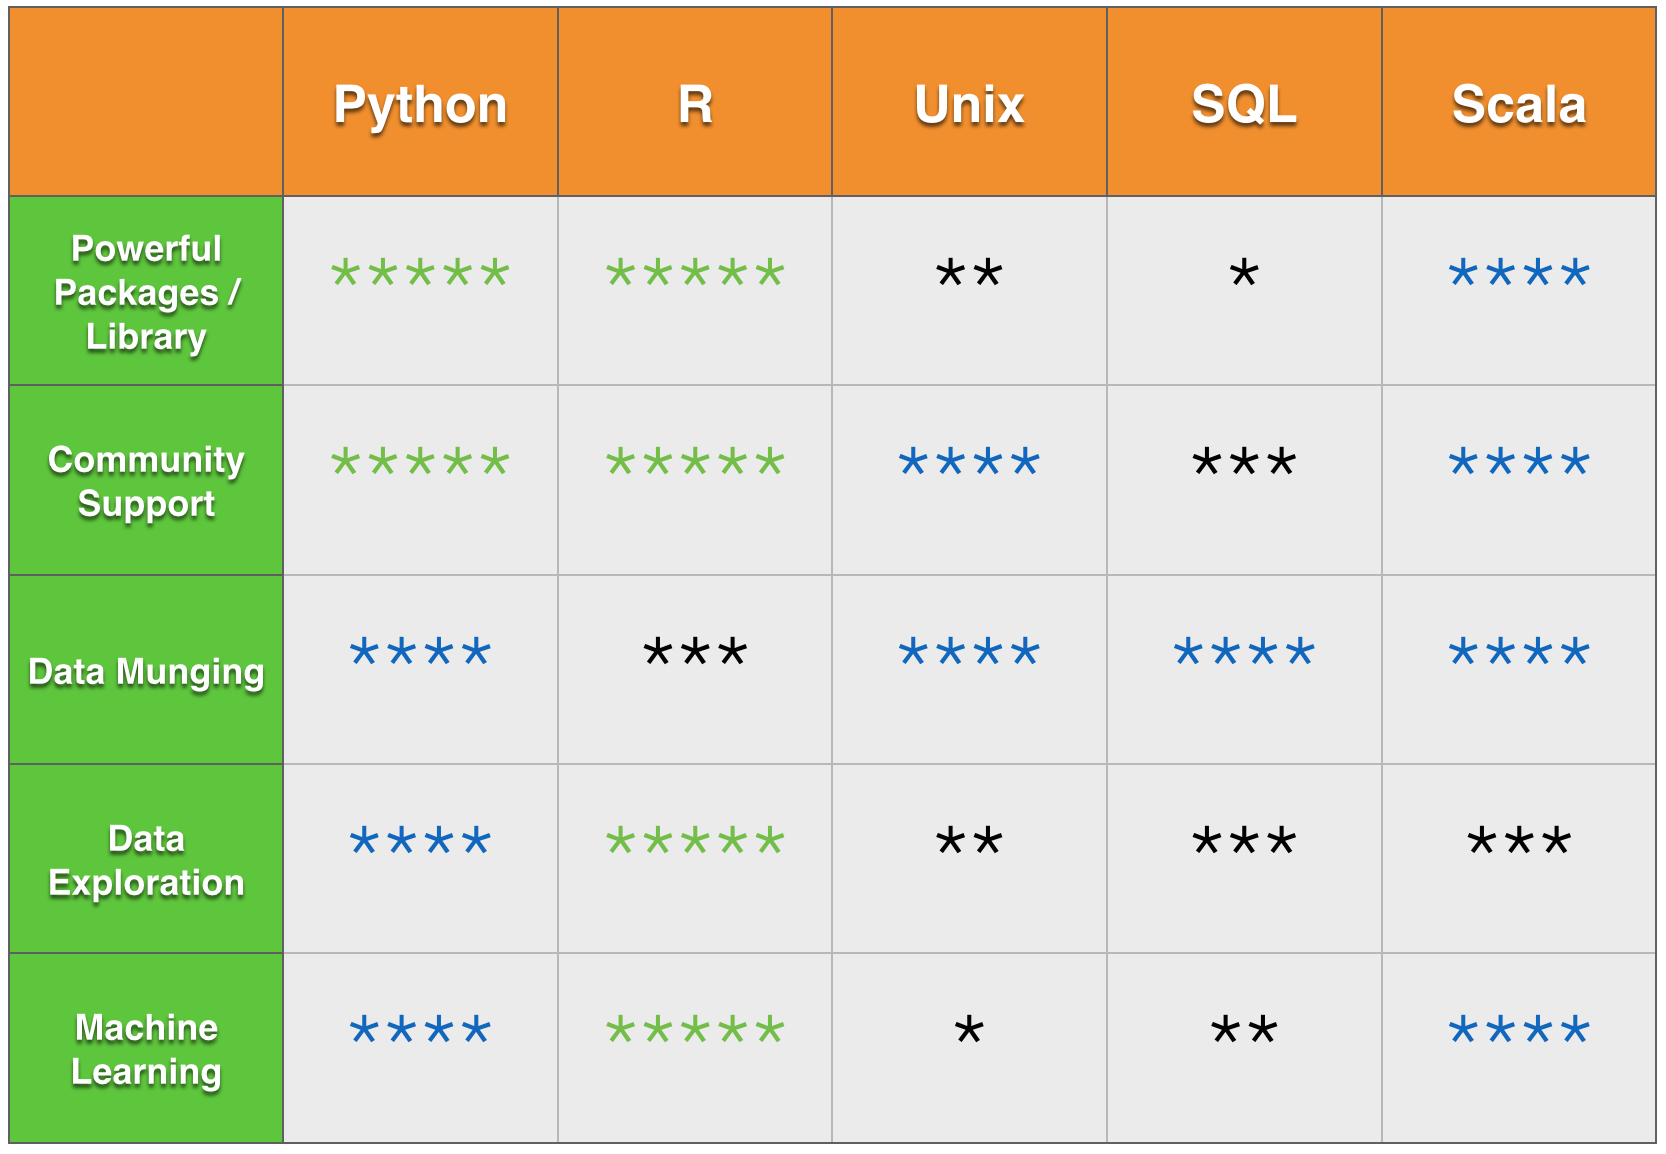
\includegraphics[width=250pt]{../graphs/data_tools}
      \end{center}
    \end{frame}

    \begin{frame}{Data visualization tools}
      \begin{center}
         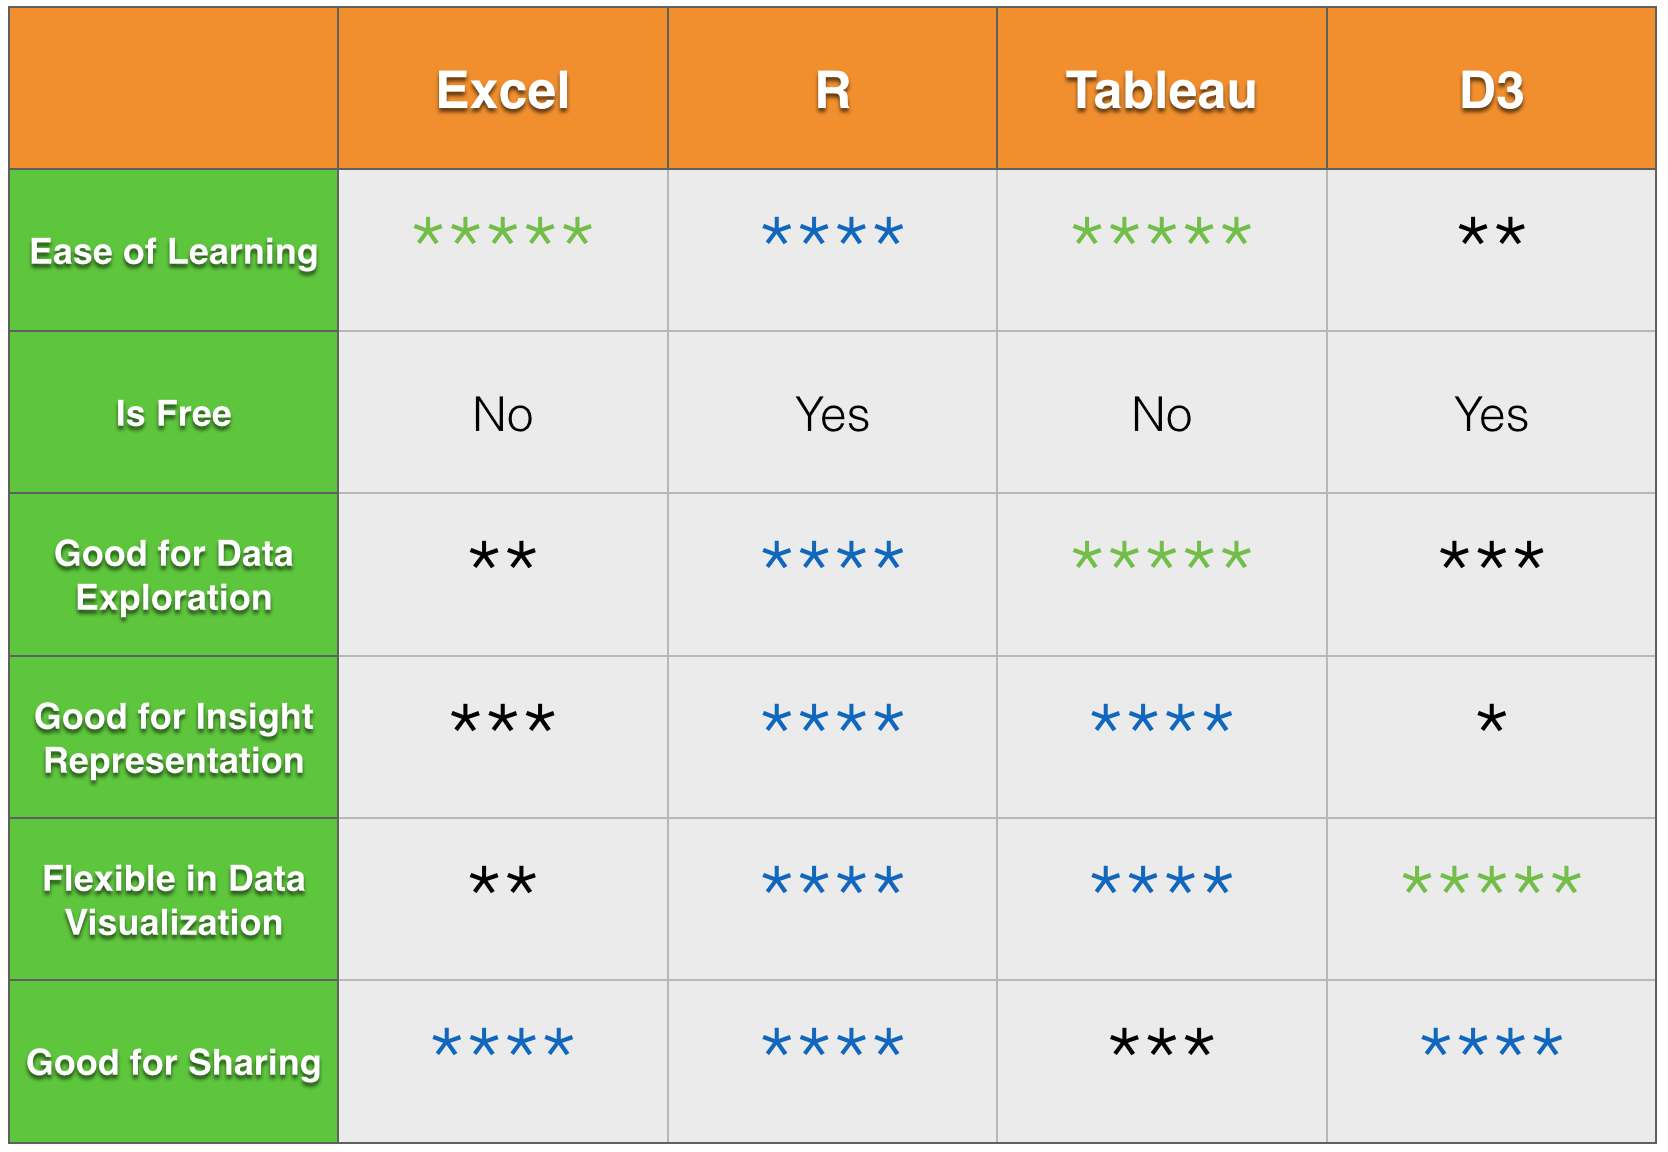
\includegraphics[width=250pt]{../graphs/data_visualization_tools}
      \end{center}
      {\footnotesize
        D3 \url{http://d3js.org/}
      }
    \end{frame}

  \subsection{Data Democracy and Big Data}

    \begin{frame}{Data Democracy}
          \begin{center}
             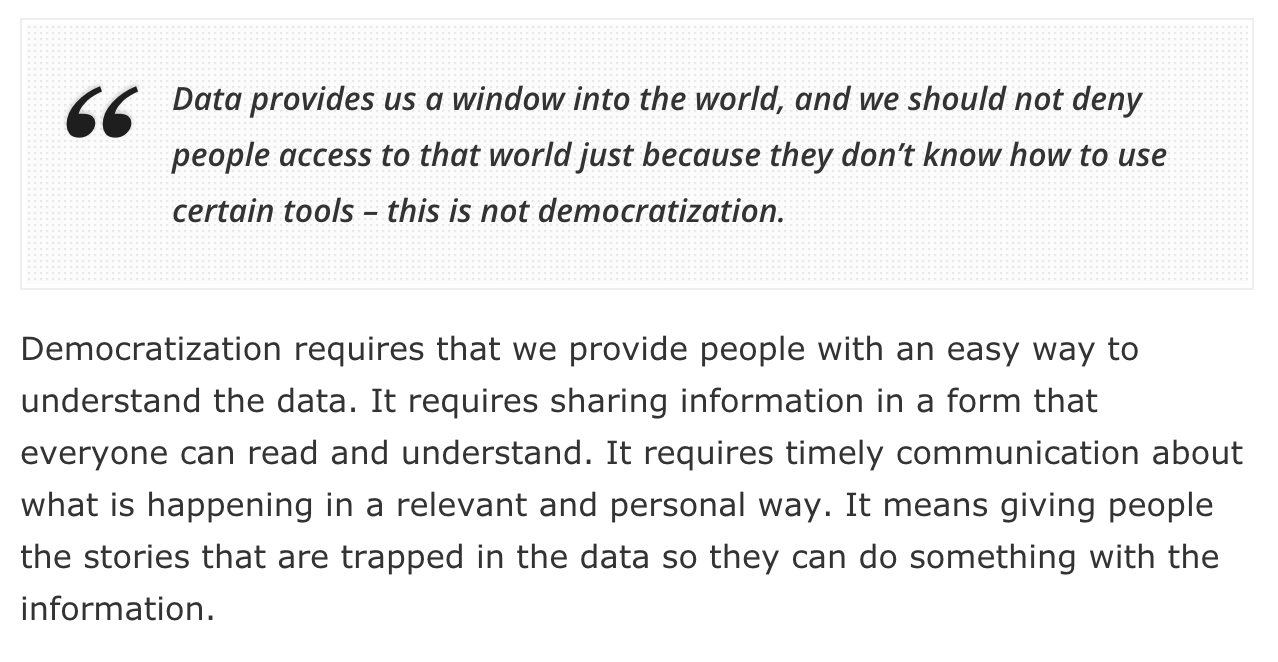
\includegraphics[width=250pt]{../graphs/data_democratization}
          \end{center}
        {\footnotesize \url{http://www.narrativescience.com/blog/democratization-data/}}
    \end{frame}

    \begin{frame}{Big Data}
      \begin{columns}
        \begin{column}[T]{0.48\textwidth}
          \begin{block}{Big Data Ecosystem}
            \begin{itemize}
              \item<1-> Hadoop - file system
              \item<2-> Spark - computing system
              \item<3-> Spark Stack
                \begin{itemize}
                  \item<4-> Spark SQL - Data Munging
                  \item<4-> Spark Streaming - Real Time Processing
                  \item<4-> MLlib - Machine Learning
                  \item<4-> GraphX - Visualization
                \end{itemize}
            \end{itemize}
          \end{block}
        \end{column}
        \begin{column}[T]{0.48\textwidth}
          \begin{overprint}
            \onslide<1>
            
\includegraphics[width=160pt]{../graphs/logo/hadoop}
            \onslide<2>
            
\includegraphics[width=160pt]{../graphs/logo/spark}
            \onslide<3->
            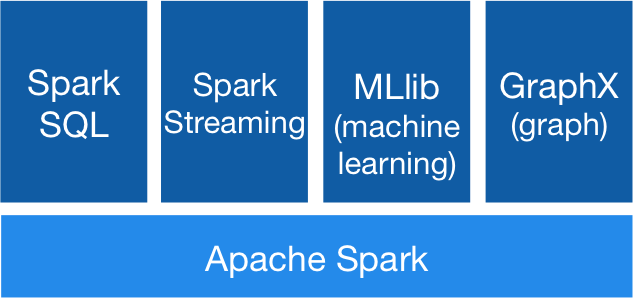
\includegraphics[width=160pt]{../graphs/logo/spark-stack}
            
            {\footnotesize \url{https://spark.apache.org/}}
          \end{overprint}
        \end{column}   
      \end{columns}
    \end{frame}

    \begin{frame}{Thank You}
      \centerline{\large Please send your questions and feedback to me!}
    \end{frame}

\end{document}